\documentclass[11pt,a4paper]{article}

\usepackage[T1]{fontenc}
\usepackage[utf8]{inputenc}
\usepackage{lmodern}
\IfFileExists{spanish.ldf}
  {\usepackage[spanish,es-noshorthands,es-tabla]{babel}}
  {\usepackage{babel}\babelprovide[import,main]{spanish}}
\usepackage[margin=2.2cm]{geometry}
\usepackage{microtype}
\usepackage{amsmath,amssymb}
\usepackage{graphicx}
\usepackage{array,booktabs,tabularx,longtable,multirow}
\usepackage[table]{xcolor}
\usepackage{enumitem}
\usepackage{titlesec}
\usepackage{fancyhdr}
\usepackage[most]{tcolorbox}
\usepackage[numbers,sort&compress]{natbib}
\usepackage[hidelinks]{hyperref}
\graphicspath{{../figuras/}}

% ---------- Estilo: una sola familia tipográfica, grises sobrios ----------
\definecolor{grisborde}{gray}{0.45}
\definecolor{grisfondo}{gray}{0.95}
\definecolor{grisfila}{gray}{0.91}

\titleformat{\section}{\normalfont\large\bfseries}{\thesection.}{0.6em}{}
\titleformat{\subsection}{\normalfont\normalsize\bfseries}{\thesubsection}{0.6em}{}
\titleformat{\subsubsection}{\normalfont\normalsize\itshape}{\thesubsubsection}{0.6em}{}
\titlespacing*{\section}{0pt}{1.2em}{0.6em}

\newtcolorbox{recuadro}[1][]{enhanced,breakable,colback=grisfondo,colframe=grisborde,
  boxrule=0.5pt,arc=1pt,left=6pt,right=6pt,top=4pt,bottom=4pt,
  fonttitle=\normalfont\bfseries,coltitle=black,colbacktitle=grisfila,#1}
\newtcolorbox{pregunta}{enhanced,breakable,colback=white,colframe=black,
  boxrule=0.8pt,arc=0pt,left=6pt,right=6pt,top=4pt,bottom=4pt}

\setlist{itemsep=1pt,topsep=3pt}
\setlength{\parindent}{0pt}
\setlength{\parskip}{4pt}
\setlength{\emergencystretch}{2em}
\renewcommand{\arraystretch}{1.18}

\setlength{\headheight}{14pt}
\pagestyle{fancy}\fancyhf{}
\lhead{\small MT227 Control Moderno y Óptimo — 2026-2}
\rhead{\small \TipoDoc{} — Encargo \Encargo}
\cfoot{\small\thepage}
\renewcommand{\headrulewidth}{0.4pt}

\newcommand{\tr}{\operatorname{tr}}
\newcommand{\sat}{\operatorname{sat}}
\newcommand{\Encargo}{E1}
\newcommand{\TipoDoc}{Informe técnico}
\newcommand{\TituloEncargo}{La ecuación de Riccati y el diseño de las ponderaciones}

% Números citados (generado por generar_results.m desde results.json)
% Generado automáticamente por generar_results.m desde results.json (clave valores_informe). No editar a mano.
\providecommand{\V}[1]{\ifcsname val@#1\endcsname\csname val@#1\endcsname\else\textbf{??\detokenize{#1}??}\fi}
\expandafter\def\csname val@m_A_kit\endcsname{1.8\times10^{-16}}
\expandafter\def\csname val@m_A_jac\endcsname{9.0\times10^{-13}}
\expandafter\def\csname val@m_polo_e\endcsname{-7240.6}
\expandafter\def\csname val@m_sep_polo\endcsname{411}
\expandafter\def\csname val@m_EL\endcsname{2.0\times10^{-16}}
\expandafter\def\csname val@p1_MF_margin\endcsname{65.5292}
\expandafter\def\csname val@p1_MF_margin_dif\endcsname{1\times10^{-3}}
\expandafter\def\csname val@p1_GM_margin\endcsname{0.4142}
\expandafter\def\csname val@p1_err_escalar\endcsname{2.2\times10^{-16}}
\expandafter\def\csname val@p1_MF_q1\endcsname{65.5302}
\expandafter\def\csname val@p1_MF_qmin\endcsname{60.0000}
\expandafter\def\csname val@p1_gmin_qmin\endcsname{0.50000}
\expandafter\def\csname val@p2_err_kit_max\endcsname{2.4\times10^{-12}}
\expandafter\def\csname val@p2_err_icare_max\endcsname{2.4\times10^{-12}}
\expandafter\def\csname val@p2_K_vs_K0\endcsname{5.4\times10^{-14}}
\expandafter\def\csname val@p2_nk_res6\endcsname{1.7\times10^{-3}}
\expandafter\def\csname val@p2_nk_res7\endcsname{3.6\times10^{-5}}
\expandafter\def\csname val@p2_nk_res8\endcsname{1.2\times10^{-8}}
\expandafter\def\csname val@p2_nk_res9\endcsname{1.2\times10^{-15}}
\expandafter\def\csname val@e11_difmax_base\endcsname{2.5\times10^{-12}}
\expandafter\def\csname val@e11_err_ham_base\endcsname{9.6\times10^{-15}}
\expandafter\def\csname val@e11_err_schur_base\endcsname{2.4\times10^{-12}}
\expandafter\def\csname val@e11_err_nk_base\endcsname{1.0\times10^{-13}}
\expandafter\def\csname val@e11_err_schur_5est\endcsname{7.2\times10^{-9}}
\expandafter\def\csname val@e11_mineigP_5est\endcsname{7.4\times10^{-14}}
\expandafter\def\csname val@e11_err_ac_max\endcsname{5.7\times10^{-12}}
\expandafter\def\csname val@e11_err_b_max_4est\endcsname{7.6\times10^{-11}}
\expandafter\def\csname val@e12_nLinv_pend\endcsname{86}
\expandafter\def\csname val@e12_cota_max\endcsname{6.9\times10^{-10}}
\expandafter\def\csname val@e12_err_real_max\endcsname{2.4\times10^{-12}}
\expandafter\def\csname val@e12_res_max\endcsname{1.4\times10^{-13}}
\expandafter\def\csname val@e12_asim_max\endcsname{1.9\times10^{-13}}
\expandafter\def\csname val@e12_mineigP\endcsname{3.4\times10^{-4}}
\expandafter\def\csname val@e12_maxRe_cl\endcsname{-2.668}
\expandafter\def\csname val@e12_nLinv_epsmin\endcsname{7.07\times10^{5}}
\expandafter\def\csname val@e12_res_peor_epsmin\endcsname{7.1\times10^{-9}}
\expandafter\def\csname val@e12_res_azar_epsmin\endcsname{3.4\times10^{-3}}
\expandafter\def\csname val@e12_disc_min\endcsname{0.7}
\expandafter\def\csname val@e12_disc_max\endcsname{0.7}
\expandafter\def\csname val@e12_icare_epsmax\endcsname{1.8\times10^{-14}}
\expandafter\def\csname val@e12_icare_epsmin\endcsname{2.1\times10^{-6}}
\expandafter\def\csname val@e13_n_problemas\endcsname{39}
\expandafter\def\csname val@e13_ref_correccion\endcsname{3.4\times10^{-42}}
\expandafter\def\csname val@e13_P3_ham\endcsname{3.6\times10^{-9}}
\expandafter\def\csname val@e13_P3_schur\endcsname{1.2\times10^{-4}}
\expandafter\def\csname val@e13_P3_pend_ham\endcsname{-0.85}
\expandafter\def\csname val@e13_P3_pend_schur\endcsname{-1.17}
\expandafter\def\csname val@e13_F1_cifras\endcsname{12}
\expandafter\def\csname val@e13_F2_schur_smax\endcsname{3.0\times10^{-2}}
\expandafter\def\csname val@e13_F2_cifras\endcsname{14}
\expandafter\def\csname val@e13_F3_max\endcsname{2.4\times10^{-12}}
\expandafter\def\csname val@e13_condU11_peor\endcsname{4.0}
\expandafter\def\csname val@e13_nk_cociente6\endcsname{0.81}
\expandafter\def\csname val@e13_nk_cociente7\endcsname{1.03}
\expandafter\def\csname val@e13_nk_cociente8\endcsname{1.07}
\expandafter\def\csname val@e13b_F1_hambal_Rmin\endcsname{3.6\times10^{-9}}
\expandafter\def\csname val@e13b_F2_bal_peor\endcsname{1.9\times10^{-13}}
\expandafter\def\csname val@e13b_P11_schur_max\endcsname{1.1\times10^{-7}}
\expandafter\def\csname val@e13b_P11_nk_max\endcsname{2.6\times10^{-9}}
\expandafter\def\csname val@e13d_F1_N3_peor\endcsname{5.3\times10^{-8}}
\expandafter\def\csname val@e13e_F3_haz_max\endcsname{8.8\times10^{-10}}
\expandafter\def\csname val@e13e_F3_nosc_max\endcsname{8.8\times10^{-10}}
\expandafter\def\csname val@e13e_F2_haz_s5\endcsname{6.4\times10^{-5}}
\expandafter\def\csname val@e13e_F2_nosc_s5\endcsname{6.3\times10^{-5}}
\expandafter\def\csname val@e13e_F2_nosc_fallos\endcsname{1}
\expandafter\def\csname val@e13e_F1_hazSx_peor\endcsname{9.8\times10^{-14}}
\expandafter\def\csname val@e13e_F1_icare_peor\endcsname{2.6\times10^{-13}}
\expandafter\def\csname val@e13e_F2_hazSx_peor\endcsname{8.4\times10^{-15}}
\expandafter\def\csname val@e13e_F2_icare_peor\endcsname{7.4\times10^{-15}}
\expandafter\def\csname val@e13e_F3_hazSx_peor\endcsname{1.6\times10^{-14}}
\expandafter\def\csname val@e13e_F3_icare_peor\endcsname{2.0\times10^{-14}}
\expandafter\def\csname val@e13e_hazSx_peor\endcsname{9.8\times10^{-14}}
\expandafter\def\csname val@e13e_D6_2\endcsname{6\times10^{-8}}
\expandafter\def\csname val@e14_N\endcsname{625}
\expandafter\def\csname val@e14_n_estables\endcsname{625}
\expandafter\def\csname val@e14_n_nd\endcsname{625}
\expandafter\def\csname val@e14_Jth_min\endcsname{8.96\times10^{-3}}
\expandafter\def\csname val@e14_Jth_max\endcsname{2.23\times10^{2}}
\expandafter\def\csname val@e14_Jal_min\endcsname{2.03\times10^{-3}}
\expandafter\def\csname val@e14_Jal_max\endcsname{0.141}
\expandafter\def\csname val@e14_Ju_min\endcsname{1.56\times10^{-3}}
\expandafter\def\csname val@e14_Ju_max\endcsname{1.11}
\expandafter\def\csname val@e14_ok_C1\endcsname{625}
\expandafter\def\csname val@e14_ok_C2_ideal\endcsname{147}
\expandafter\def\csname val@e14_ok_C2_real\endcsname{115}
\expandafter\def\csname val@e14_ok_C2_real_sat\endcsname{101}
\expandafter\def\csname val@e14_sensor_falla\endcsname{48}
\expandafter\def\csname val@e14_cambian\endcsname{64}
\expandafter\def\csname val@e14_dif_lyap\endcsname{1.3\times10^{-9}}
\expandafter\def\csname val@e14_dif_suma\endcsname{1.9\times10^{-10}}
\expandafter\def\csname val@e14_dif_ode\endcsname{2.3\times10^{-11}}
\expandafter\def\csname val@e14_n_ode\endcsname{10}
\expandafter\def\csname val@e14_dif_solver\endcsname{8.9\times10^{-11}}
\expandafter\def\csname val@e14_base_C1_uc\endcsname{9.12}
\expandafter\def\csname val@e14_base_C2_th\endcsname{1.237}
\expandafter\def\csname val@e14_base_C2r_uc\endcsname{63.82}
\expandafter\def\csname val@e14_base_C2r_th\endcsname{1.345}
\expandafter\def\csname val@e14_spearman\endcsname{0.960}
\expandafter\def\csname val@e15_sigma_min\endcsname{0.458}
\expandafter\def\csname val@e15_fmin_desde_base\endcsname{0.9625}
\expandafter\def\csname val@e15_fmin_desde_malla\endcsname{0.9614}
\expandafter\def\csname val@e15_Jrel_semilla1\endcsname{0.961}
\expandafter\def\csname val@e15_val_Jrel\endcsname{0.9945}
\expandafter\def\csname val@e15_val_Jrel_desv\endcsname{0.019}
\expandafter\def\csname val@e15_ts_C1_max\endcsname{0.132}
\expandafter\def\csname val@e15_P2_K2_base\endcsname{182.5}
\expandafter\def\csname val@e15_P2_m_falla\endcsname{17.8}
\expandafter\def\csname val@e15_P2_K2_falla\endcsname{60}
\expandafter\def\csname val@e15b_r_th\endcsname{1.58}
\expandafter\def\csname val@e15b_r_al\endcsname{1}
\expandafter\def\csname val@e15b_Jrel_base_malla\endcsname{0.9991}
\expandafter\def\csname val@e15b_saa_Jrel\endcsname{0.9994}
\expandafter\def\csname val@e15b_saa_Jrel_desv\endcsname{0.0225}
\expandafter\def\csname val@e15b_saa_t\endcsname{0.12}
\expandafter\def\csname val@e15b_saa_mej_C1\endcsname{-1.2}
\expandafter\def\csname val@e15b_saa_t_C1\endcsname{-4.5}
\expandafter\def\csname val@e15b_saa_mej_C2\endcsname{1.5}
\expandafter\def\csname val@e15b_saa_t_C2\endcsname{45.8}
\expandafter\def\csname val@e15b_s1_mej_C1\endcsname{-8.2}
\expandafter\def\csname val@e15b_s1_mej_C3b\endcsname{5.2}
\expandafter\def\csname val@e15b_s1_t_C3b\endcsname{8.3}
\expandafter\def\csname val@e15c_piso_C1\endcsname{0.55}
\expandafter\def\csname val@e15c_piso_C2\endcsname{0.01}
\expandafter\def\csname val@e15c_piso_C3\endcsname{3.1}
\expandafter\def\csname val@e15c_piso_C3b\endcsname{0.09}
\expandafter\def\csname val@e15c_piso_ideal_max\endcsname{6\times10^{-16}}
\expandafter\def\csname val@e15d_K_lmi_vs_K0\endcsname{1.3\times10^{-4}}
\expandafter\def\csname val@e15d_J_lmi_libre\endcsname{1.000000}
\expandafter\def\csname val@e15d_costo_region\endcsname{2.5}
\expandafter\def\csname val@e15d_sigma_g\endcsname{2.939}
\expandafter\def\csname val@e15d_zeta_g\endcsname{0.885}
\expandafter\def\csname val@e15d_base_sigma\endcsname{2.668}
\expandafter\def\csname val@e15d_base_zeta\endcsname{0.742}
\expandafter\def\csname val@e15d_s4_Q\endcsname{1.18}
\expandafter\def\csname val@e15d_s4_LMI\endcsname{1.57}
\expandafter\def\csname val@e15d_s6_Q\endcsname{1.46}
\expandafter\def\csname val@e15d_s6_LMI\endcsname{2.79}
\expandafter\def\csname val@e15d_z85_Q\endcsname{1.48}
\expandafter\def\csname val@e15d_z85_LMI\endcsname{1.18}
\expandafter\def\csname val@e15d_z90_Q\endcsname{1.98}
\expandafter\def\csname val@e15d_z90_LMI\endcsname{1.25}
\expandafter\def\csname val@e15d_n_casos\endcsname{16}
\expandafter\def\csname val@e15d_n_region_ok\endcsname{16}
\expandafter\def\csname val@e15d_n_cota_ok\endcsname{16}
\expandafter\def\csname val@e15d_s4_C2_sat_ideal\endcsname{99.9}
\expandafter\def\csname val@e15d_5sem_Jrel\endcsname{0.977}
\expandafter\def\csname val@e15d_5sem_desv\endcsname{0.009}
\expandafter\def\csname val@e15d_5sem_mejora\endcsname{2.3}
\expandafter\def\csname val@e15d_val_ok\endcsname{20}
\expandafter\def\csname val@e15d_val_Jrel\endcsname{0.9982}
\expandafter\def\csname val@e15d_val_Jrel_desv\endcsname{0.0216}
\expandafter\def\csname val@e15d_val_t\endcsname{0.37}
\expandafter\def\csname val@e15d_val_mej_C1\endcsname{-6.6}
\expandafter\def\csname val@e15d_val_mej_C2\endcsname{-3.2}
\expandafter\def\csname val@e15d_val_mej_C3b\endcsname{7.6}
\expandafter\def\csname val@e16_rho\endcsname{1.635\times10^{-2}}
\expandafter\def\csname val@e16_corte_theta\endcsname{0.144}
\expandafter\def\csname val@e16_corte_alpha\endcsname{0.0377}
\expandafter\def\csname val@e16_franja\endcsname{0.055}
\expandafter\def\csname val@e16_al_emp\endcsname{0.430}
\expandafter\def\csname val@e16_rad_ideal_exito\endcsname{0.388}
\expandafter\def\csname val@e16_rad_oficial_exito\endcsname{0.378}
\expandafter\def\csname val@e16_rad_oficial_rec\endcsname{0.457}
\expandafter\def\csname val@e16_efecto_sensor\endcsname{-2.4}
\expandafter\def\csname val@e16_P1_razon_id\endcsname{11}
\expandafter\def\csname val@e16_P1_razon_of\endcsname{10}
\expandafter\def\csname val@e16_razon_min\endcsname{8.5}
\expandafter\def\csname val@e16_razon_max\endcsname{31.9}
\expandafter\def\csname val@e16_razon_med\endcsname{12.2}
\expandafter\def\csname val@e16_n_dir\endcsname{200}
\expandafter\def\csname val@e16_mc_N\endcsname{20\,000}
\expandafter\def\csname val@e16_mc_rec\endcsname{44.8}
\expandafter\def\csname val@e16_mc_exito\endcsname{34.6}
\expandafter\def\csname val@e16_C2_margen\endcsname{0.028}
\expandafter\def\csname val@e16_max_Kx\endcsname{9.996}
\expandafter\def\csname val@e16_dV_neg\endcsname{100}
\expandafter\def\csname val@e16_rango_obs\endcsname{4}
\expandafter\def\csname val@e16_in_rec\endcsname{5000}
\expandafter\def\csname val@e16_in_n\endcsname{5000}
\expandafter\def\csname val@e16_in_max_uc\endcsname{9.815}
\expandafter\def\csname val@e16_in_sat\endcsname{0}
\expandafter\def\csname val@e16_lote_coinc\endcsname{60}
\expandafter\def\csname val@e16_lote_n\endcsname{60}
\expandafter\def\csname val@e16_lote_dif\endcsname{1.5\times10^{-19}}
\expandafter\def\csname val@e16_vol_razon\endcsname{5506}
\expandafter\def\csname val@e16_radio_theta\endcsname{4.6}
\expandafter\def\csname val@esc_C2_sat\endcsname{1.9}
\expandafter\def\csname val@esc_C2_th\endcsname{1.345}

\begin{document}
\noindent
\begin{minipage}[c]{0.17\linewidth}
  \IfFileExists{logo_uni.png}{
\includegraphics[width=\linewidth]{logo_uni.png}}{}
\end{minipage}\hfill
\begin{minipage}[c]{0.79\linewidth}
  \centering
  {\large\bfseries UNIVERSIDAD NACIONAL DE INGENIERÍA}\\[2pt]
  {\normalsize MT227C — Control Moderno y Óptimo — 2026-2}\\[8pt]
  {\Large\bfseries \TipoDoc{} — Encargo \Encargo}\\[4pt]
  {\large \TituloEncargo}
\end{minipage}

\vspace{1em}
\begin{center}\small
\begin{tabularx}{\linewidth}{@{}l l X@{}}
\toprule
Integrante & Código & Subsección de la que es responsable \\
\midrule
Zamudio Salazar, Joseluis Omar & 20193529C & E1.4--E1.6 (Pareto, optimización con restricciones y LMI, región de atracción), escenarios C1--C4 y repositorio \\
Nava Laburiano, David Adrián & 20211012C & E1.1--E1.3 (métodos de Riccati, verificación y estrés numérico); verificación cruzada de los códigos \\
\bottomrule
\end{tabularx}
\end{center}

\begin{pregunta}
\textbf{Pregunta de investigación.} ¿Qué método de solución de la ecuación algebraica de Riccati es
confiable para esta planta, cuándo deja de serlo, y cómo se traducen especificaciones físicas en
$(Q,R)$ con garantías verificables sobre la planta no lineal y saturada?
\end{pregunta}

\section*{Resumen}
Para el péndulo de Furuta los tres métodos de solución de la ecuación de Riccati coinciden con
\texttt{icare} dentro de $\V{e11_err_schur_base}$ en el diseño base, pero la confiabilidad no la decide el método:
la decide el escalado de los datos. Sin equilibrado, los métodos de subespacio pierden hasta
$\V{e13_F1_cifras}$ cifras con $R=10^{-8}$ y $\V{e13_F2_cifras}$ al cambiar las unidades de las velocidades, mientras que el haz
extendido con escalado de estados y entrada mantiene un error $\le\V{e13e_hazSx_peor}$ en los
$\V{e13_n_problemas}$ problemas de estrés; y un residuo pequeño solo certifica un error pequeño cuando
$\|\mathcal L^{-1}\|$ es moderado ($\V{e12_nLinv_pend}$ en el péndulo, frente a $\V{e12_nLinv_epsmin}$ en un caso construido).
Las especificaciones (decaimiento $\sigma\ge\V{e15_sigma_min}$~s$^{-1}$, $\zeta\ge0.5$, $|\theta|\le\pi/2$ y saturación
$\le5\,\%$ en C2) se traducen en $(Q,R)$ con un problema de dos niveles evaluado en el simulador oficial: el
diseño base las cumple y ningún otro LQR lo mejora de forma significativa en semillas independientes
($J_{rel}=\V{e15b_saa_Jrel}\pm\V{e15b_saa_Jrel_desv}$, $t=\V{e15b_saa_t}$). La garantía verificable es un elipsoide de
$\V{e16_corte_alpha}$~rad sobre $\alpha$, mientras que el Monte Carlo no lineal recupera el péndulo desde
$\V{e16_al_emp}$~rad: lo certificado es entre $\V{e16_razon_min}$ y $\V{e16_razon_max}$ veces menor que lo estimado.

\tableofcontents

% =====================================================================
\section{Introducción y estado del arte}
El regulador lineal cuadrático (LQR) minimiza $J=\int_0^\infty (x^\top Qx+u^\top Ru)\,dt$ con $u=-Kx$,
$K=R^{-1}B^\top P$, donde $P=P^\top\succeq0$ es la solución estabilizante de la ecuación algebraica de Riccati
\begin{equation}
\mathcal R(P)=A^\top P+PA-PSP+Q=0,\qquad S=BR^{-1}B^\top ,\label{eq:are}
\end{equation}
que existe y es única si $(A,B)$ es estabilizable y $(A,Q^{1/2})$ es detectable. Hay tres familias clásicas de
solución. Potter \cite{potter1966} obtuvo $P$ de los vectores propios de la matriz Hamiltoniana
$H=\left[\begin{smallmatrix}A&-S\\-Q&-A^\top\end{smallmatrix}\right]$ asociados a sus $n$ autovalores estables;
Laub \cite{laub1979} reemplazó esos vectores por una base ortogonal del mismo subespacio, obtenida de la forma real
de Schur ordenada, lo que evita la mala condición de los vectores propios cuando hay autovalores cercanos;
y Kleinman \cite{kleinman1968} propuso una iteración de Newton que resuelve una ecuación de Lyapunov por paso
(por ejemplo, con el método de Bartels y Stewart \cite{bartels1972}) y converge cuadráticamente desde una
ganancia estabilizante, que puede obtenerse con el algoritmo de Bass \cite{armstrong1975}. Van Dooren
\cite{vandooren1981} y Arnold y Laub \cite{arnold1984} formularon el problema como un haz de matrices
extendido que no exige formar $S$, y propusieron equilibrar los datos; \texttt{icare} de MATLAB usa un haz de
este tipo con escalado de estados y entrada \cite{mathworks2026}.

La calidad de una solución calculada se juzga con dos medidas distintas: el residuo $\mathcal R(\hat P)$ (error
inverso) y el error directo $\|\hat P-P\|/\|P\|$, que se relacionan mediante el condicionamiento del problema
\cite{higham2002}. Kenney, Laub y Wette \cite{kenney1990} dieron cotas del error de una solución aproximada a
partir del residuo y del operador de Lyapunov del lazo cerrado, y Sun \cite{sun1998} desarrolló la teoría de
perturbaciones de la ecuación \eqref{eq:are}. En el lado del diseño, los pesos suelen normalizarse por el
cuadrado del valor máximo admisible de cada variable \cite{bryson2018}, y el compromiso entre objetivos
cuadráticos se explora por escalarización con pesos positivos, que da puntos Pareto-óptimos \cite{marler2004}.
Cuando el costo se evalúa en un simulador con ruido, optimizar con una sola realización sobreestima la mejora
\cite{smith2006}; la aproximación por promedio muestral (SAA) con validación independiente es la respuesta
estándar \cite{kleywegt2002}. Las especificaciones de polos (decaimiento y amortiguamiento) pueden imponerse
como regiones LMI con una matriz de Lyapunov común \cite{chilali1996,boyd1994}. Con un actuador saturado,
la estabilidad del lazo es solo local: los conjuntos de nivel de una función de Lyapunov cuadrática contenidos
en la región lineal del actuador dan una estimación certificada pero conservadora de la región de atracción
\cite{hu2001}, y el principio de invariancia de LaSalle \cite{lasalle1960} permite concluir convergencia cuando la
derivada de la función es solo semidefinida.

El péndulo rotatorio de Furuta \cite{furuta1992} es un banco de pruebas habitual, con un modelo de
Euler--Lagrange bien establecido \cite{cazzolato2011} y una plataforma comercial (QUBE-Servo 2) con parámetros
publicados \cite{quanser2016}. Lo que la literatura no responde para esta planta concreta es qué método es
confiable con sus escalas reales (un polo eléctrico a $\V{m_polo_e}$~rad/s, ángulos en radianes y tensiones en voltios),
dónde deja de serlo y cómo se traducen especificaciones físicas en $(Q,R)$ cuando la planta satura y se mide con
encoders cuantizados. Este trabajo aporta: (i) la comparación de los tres métodos en los mismos problemas y su
verificación frente a una referencia en precisión extendida; (ii) la identificación del escalado, y no del método,
como causa de la pérdida de precisión; (iii) un diseño de pesos validado estadísticamente en el simulador oficial;
y (iv) la cuantificación de la distancia entre la región de atracción certificada y la estimada.

% =====================================================================
\section{Modelo y simulador}
\paragraph{Modelo no lineal.} Con $x=[\theta\;\alpha\;\dot\theta\;\dot\alpha]^\top$ ($\alpha=0$: péndulo arriba) y
$q=[\theta\;\alpha]^\top$, el brazo (inercia $J_r$ respecto del pivote, longitud $r$) y el péndulo (varilla uniforme de
masa $m_p$, longitud $L_p$, $l_p=L_p/2$, $J_p=m_pL_p^2/3$) tienen energía cinética
$T=\tfrac12\dot q^\top M(\alpha)\dot q$ y potencial $V=m_pgl_p\cos\alpha$, con
\begin{equation}
M(\alpha)=\begin{bmatrix}J_r+m_pr^2+J_p\sin^2\alpha & -m_prl_p\cos\alpha\\ -m_prl_p\cos\alpha & J_p\end{bmatrix}.
\end{equation}
Las ecuaciones de Euler--Lagrange \cite{cazzolato2011}, con amortiguamientos viscosos $D_r$ y $D_p$, son
\begin{equation}
M(\alpha)\ddot q=\begin{bmatrix}\tau-D_r\dot\theta-2J_p\sin\alpha\cos\alpha\,\dot\theta\dot\alpha-m_prl_p\sin\alpha\,\dot\alpha^2\\
m_pgl_p\sin\alpha+J_p\sin\alpha\cos\alpha\,\dot\theta^2-D_p\dot\alpha\end{bmatrix},
\end{equation}
con el par del motor $\tau=k_t\,i_a$ y el circuito de armadura $L_m\,di_a/dt=V_m-R_mi_a-k_m\dot\theta$.
Los parámetros son los de \texttt{parametros\_qube} del kit (manual QUBE-Servo 2, tabla 2.2 \cite{quanser2016};
$D_r$ y $D_p$ son supuestos de modelo declarados por el kit). La matriz de masa se dedujo además de forma
simbólica desde la geometría (\texttt{modelo\_propio.m}).

\paragraph{Reducción a 4 estados.} El modelo de 5 estados ($x_e=[x^\top\;i_a]^\top$) tiene un polo eléctrico en
$\V{m_polo_e}$~rad/s, $\V{m_sep_polo}$ veces más rápido que el polo mecánico más rápido. Por perturbación singular
($L_m\to0$) la corriente sigue a la tensión, $i_a\approx(V_m-k_m\dot\theta)/R_m$, y queda el modelo de 4 estados con
$\tau=k_t(V_m-k_m\dot\theta)/R_m$. E1.1 confirma que la reducción no cambia el regulador: el LQR de 5 estados difiere
de $K_0$ en $\V{e11_K5_dif}$ en la parte mecánica y pone una ganancia de solo $\V{e11_K5_ia}$~V/A sobre la corriente.

\paragraph{Linealización.} El jacobiano en el equilibrio superior da
\begin{equation}
A=\begin{bmatrix}0&0&1&0\\0&0&0&1\\0&\V{mod_A32}&\V{mod_A33}&\V{mod_A34}\\0&\V{mod_A42}&\V{mod_A43}&\V{mod_A44}\end{bmatrix},\qquad
B=\begin{bmatrix}0\\0\\\V{mod_B3}\\\V{mod_B4}\end{bmatrix},
\end{equation}
con $B_3,B_4>0$ (regla de signos de la guía) y autovalores $\V{mod_eigA_1}$, $\V{mod_eigA_2}$, $\V{mod_eigA_3}$ y
$\V{mod_eigA_4}$~s$^{-1}$: el modo del péndulo es inestable y $\theta$ no aparece en la dinámica (primera columna
nula). $(A,B)$ coincide con \texttt{lineal\_qube} del kit con error relativo $\V{m_A_kit}$, con el jacobiano
numérico por diferencias centrales con $\V{m_A_jac}$ y con la deducción simbólica con $\V{m_EL}$ (sección
\ref{sec:pruebas}). El diseño base del curso, $Q_0=\operatorname{diag}((\pi/4)^{-2},(\pi/36)^{-2},0,0)$ y
$R_0=10^{-2}$, da $K_0=[\V{K0_1}\;\;\V{K0_2}\;\;\V{K0_3}\;\;\V{K0_4}]$ y polos de lazo cerrado
$\V{cl_lento_re}\pm \V{cl_lento_im}j$ y $\V{cl_rapido_re}\pm \V{cl_rapido_im}j$.

\paragraph{Simulador.} Todos los resultados oficiales se obtienen con el simulador del kit v1.1.1
(sección 2.4 de la guía): integración Runge--Kutta de cuarto orden con paso de 0.5~ms, lazo digital con
$T_s=2$~ms y retención de orden cero, saturación $|u|\le V_{\max}=10$~V, encoders de 2048 cuentas por vuelta
($y=q\,\mathrm{round}(z/q)$, $q=2\pi/2048$), ruido de par blanco sobre el brazo ($S_\tau=10^{-8}$~N$^2$m$^2$s) con semilla
fija y el filtro de Kalman base $(L_0,\Sigma_0)$ para estimar las velocidades. Para los barridos masivos de E1.6 se
programó un simulador por lotes (\texttt{src/simular\_lote.m}) con la misma dinámica y el mismo lazo digital, pero
con estado exacto; se contrastó con el del kit (sección \ref{sec:e16}).

\section{Pruebas con respuesta conocida}
Scripts: \texttt{pruebas\_kit.m} (kit, 22 de 22 superadas), \texttt{modelo\_propio.m} y
\texttt{pruebas\_E1.m}.

\begin{center}\small
\begin{tabularx}{\linewidth}{@{}X l l l@{}}
\toprule
Prueba & Esperado & Obtenido & Error \\
\midrule
Modelo propio $A$ frente al kit & \texttt{lineal\_qube} & coincide & $1.8\times10^{-16}$ \\
Modelo propio $A$ frente al jacobiano numérico & diferencias centrales & coincide & $9.0\times10^{-13}$ \\
Euler--Lagrange simbólico desde la geometría & $A$, $B$ propios & coincide & $1.7\times10^{-16}$ \\
$\dot x=x+u$, $q=1$: ganancia & $K=1+\sqrt2=2.414214$ & 2.414214 & $\le1.8\times10^{-16}$ \\
$\dot x=x+u$, $q=1$: margen de fase & $65.5^\circ$ & $65.5302^\circ$ (exacto, \texttt{fzero}) & -- \\
$\dot x=x+u$, $q=1$: margen de fase con \texttt{margin} & $65.5302^\circ$ & $65.5292^\circ$ & $1\times10^{-3}$\,$^\circ$ \\
$\dot x=x+u$, $q=1$: margen de ganancia con \texttt{margin} & $1/K=0.4142$ & 0.4142 & -- \\
$\dot x=x+u$, $q\to0^+$: margen de fase & $\to60^\circ$ por encima & $60.0000^\circ$ ($q=10^{-6}$) & -- \\
$\dot x=x+u$, $q\to0^+$: ganancia mínima tolerable & $\to1/2$ & 0.50000 ($q=10^{-6}$) & -- \\
Tres solucionadores frente a $P_0$ del kit & diferencia $<10^{-10}$ & máx.\ $2.4\times10^{-12}$ & OK \\
Tres solucionadores frente a \texttt{icare} & diferencia $<10^{-10}$ & máx.\ $2.4\times10^{-12}$ & OK \\
\bottomrule
\end{tabularx}
\end{center}

La tabla resume las pruebas que la guía exige antes de trabajar con el péndulo. Todas se superan con
márgenes de varios órdenes de magnitud respecto de la tolerancia $10^{-10}$; la única diferencia mayor que el
redondeo es la de \texttt{margin}, que halla la frecuencia de cruce de forma numérica.

% =====================================================================
\section{Resultados}

\subsection{E1.1 --- Tres métodos de solución de la ecuación de Riccati}
\paragraph{Planteamiento.} Comparar, en los mismos problemas, (a) vectores propios de $H$, (b) Schur real
ordenado y (c) Newton--Kleinman, con \texttt{icare} como referencia de biblioteca. Banco de seis problemas: el
escalar $\dot x=x+u$; el diseño base; $R=100R_0$; $R=R_0/100$; $Q=I$, $R=1$; y el modelo de 5 estados con
$Q=\operatorname{diag}(Q_0,0)$.

\paragraph{Desarrollo.} (a) Si $[X_1;X_2]$ reúne los vectores propios de los $n$ autovalores de $H$ con parte real
negativa, $P=X_2X_1^{-1}$ (parte real, simetrizada al final). (b) Con $H=UTU^\top$ ordenada de modo que el bloque
$T_{11}$ contenga los autovalores estables, $P=U_{21}U_{11}^{-1}$ \cite{laub1979}. (c) Con $K_k$ estabilizante,
\begin{equation}
(A-BK_k)^\top P_k+P_k(A-BK_k)+Q+K_k^\top RK_k=0,\qquad K_{k+1}=R^{-1}B^\top P_k ,
\end{equation}
hasta que el residuo relativo baja de $10^{-12}$ o deja de disminuir. La ganancia inicial es la de Bass
\cite{armstrong1975}, $K_0^{B}=B^\top Z^{-1}$ con $(A+\beta I)Z+Z(A+\beta I)^\top=2BB^\top$ y $\beta=20>|\V{mod_eigA_1}|$; en el
modelo de 5 estados Bass exigiría $\beta$ mayor que el polo eléctrico y la ecuación de Lyapunov queda mal
condicionada, por lo que se usa $[K_0\;0]$, que es estabilizante.

\paragraph{Resultados y verificación.} En el diseño base la diferencia máxima entre los tres métodos es
$\V{e11_difmax_base}$ y los errores frente a \texttt{icare} son $\V{e11_err_ham_base}$ (a), $\V{e11_err_schur_base}$ (b) y
$\V{e11_err_nk_base}$ (c) (figura \ref{fig:e11}). En los cinco primeros problemas todos quedan bajo la tolerancia
$10^{-10}$; (b) es siempre el menos preciso (máximo $\V{e11_err_b_max_4est}$) y solo la supera en el modelo de 5
estados ($\V{e11_err_schur_5est}$), cuya $P$ es casi singular ($\lambda_{\min}(P)=\V{e11_mineigP_5est}$) porque la
corriente no se pondera y su modo es $\V{m_sep_polo}$ veces más rápido. Tres comprobaciones independientes sostienen el
resultado: $P_0$ del kit (diferencia máxima $\V{p2_err_kit_max}$), la solución analítica del caso escalar (error
$\le\V{p1_err_escalar}$) y la convergencia cuadrática de Newton--Kleinman, cuyo residuo pasa de $\V{p2_nk_res6}$ a
$\V{p2_nk_res7}$, $\V{p2_nk_res8}$ y $\V{p2_nk_res9}$ en las iteraciones 6 a 9.

\begin{figure}[h]
\centering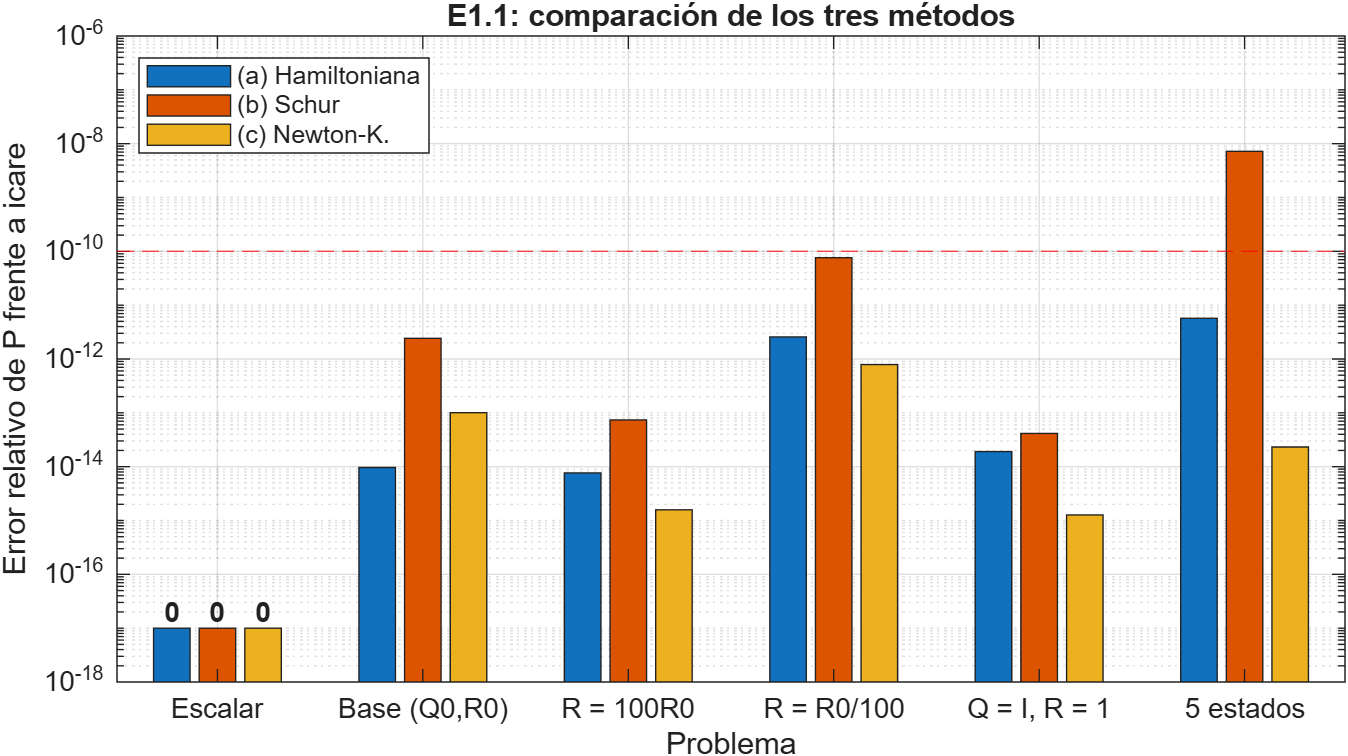
\includegraphics[width=0.78\linewidth]{E1_1_errores.png}
\caption{E1.1: error relativo de $P$ frente a \texttt{icare} por problema y método (escala logarítmica; ``0'':
coincidencia exacta). La línea discontinua es la tolerancia $10^{-10}$ de la guía.}\label{fig:e11}
\end{figure}

\paragraph{Interpretación.} Para el diseño base los tres métodos son confiables y equivalentes en la práctica:
sus diferencias son del orden de $10^{-12}$, irrelevantes frente a cualquier tolerancia de diseño. La ordenación
observada, con Schur por detrás de los vectores propios, contradice lo que predice la teoría para matrices mal
condicionadas \cite{laub1979}; E1.3 muestra que la causa no es el método sino que \texttt{eig} equilibra $H$ y
\texttt{schur} no.

\subsection{E1.2 --- Verificación de las soluciones y condicionamiento}
\paragraph{Planteamiento.} Verificar cada solución con cuatro pruebas (residuo relativo normalizado, simetría,
$P\succeq0$ y $A-BK$ Hurwitz) y mostrar, con un caso construido, que un residuo pequeño no implica un error
pequeño.

\paragraph{Desarrollo.} El residuo se normaliza como
$r=\|\mathcal R(\hat P)\|_F/(\|A^\top\hat P\|_F+\|\hat PA\|_F+\|\hat PS\hat P\|_F+\|Q\|_F)$. Si $\hat P=P^\star+\Delta$,
\begin{equation}
\mathcal R(P^\star+\Delta)=\mathcal L(\Delta)-\Delta S\Delta,\qquad \mathcal L(X)=A_c^\top X+XA_c,\quad A_c=A-SP^\star ,
\end{equation}
de modo que, a primer orden, $\|\Delta\|\lesssim\|\mathcal L^{-1}\|\,\|\mathcal R(\hat P)\|$
\cite{kenney1990}. Los autovalores de $\mathcal L=I\otimes A_c^\top+A_c^\top\otimes I$ son $\lambda_i+\lambda_j$; si $A_c$ tiene
polos cerca del eje imaginario, $\|\mathcal L^{-1}\|=1/\sigma_{\min}(\mathcal L)$ es grande y existen errores que el
residuo casi no ve. El caso construido es un oscilador sin amortiguamiento con $Q=\varepsilon^2I$, $R=1$, cuya
solución exacta es $p_2=\varepsilon^2/(1+\sqrt{1+\varepsilon^2})$, $p_3=\sqrt{2p_2+\varepsilon^2}$, $p_1=p_3(1+p_2)$, con
polos de lazo cerrado $\approx-\varepsilon/\sqrt2\pm j$. Se perturba $P^\star$ con un error relativo fijo de $1\,\%$ en dos
direcciones: la del menor valor singular de $\mathcal L$ y una aleatoria.

\paragraph{Resultados y verificación.} Con $\varepsilon=10^{-6}$, $\|\mathcal L^{-1}\|=\V{e12_nLinv_epsmin}$ y el error de
$1\,\%$ en la dirección peor produce un residuo de solo $\V{e12_res_peor_epsmin}$, mientras que la misma magnitud
en una dirección aleatoria da $\V{e12_res_azar_epsmin}$ (figura \ref{fig:e12}). La aproximación de primer orden se
comprobó fila a fila: $\mathcal R$ y $\mathcal L(\Delta)$ difieren entre $\V{e12_disc_min}\,\%$ y $\V{e12_disc_max}\,\%$, la
contribución del término cuadrático. La propia \texttt{icare} pierde precisión en este caso, de $\V{e12_icare_epsmax}$
con $\varepsilon=10^{-1}$ a $\V{e12_icare_epsmin}$ con $\varepsilon=10^{-6}$, por eso la referencia es la solución analítica.
En el péndulo, $\|\mathcal L^{-1}\|=\V{e12_nLinv_pend}$, la cota $\|\mathcal L^{-1}\|\,\|\mathcal R\|/\|P\|\le\V{e12_cota_max}$ queda por
encima del error real ($\le\V{e12_err_real_max}$) y las tres soluciones pasan las cuatro pruebas: residuo
$\le\V{e12_res_max}$, asimetría $\le\V{e12_asim_max}$, $\lambda_{\min}(P)=\V{e12_mineigP}$ y
$\max\operatorname{Re}\lambda(A-BK)=\V{e12_maxRe_cl}$.

\begin{figure}[h]
\centering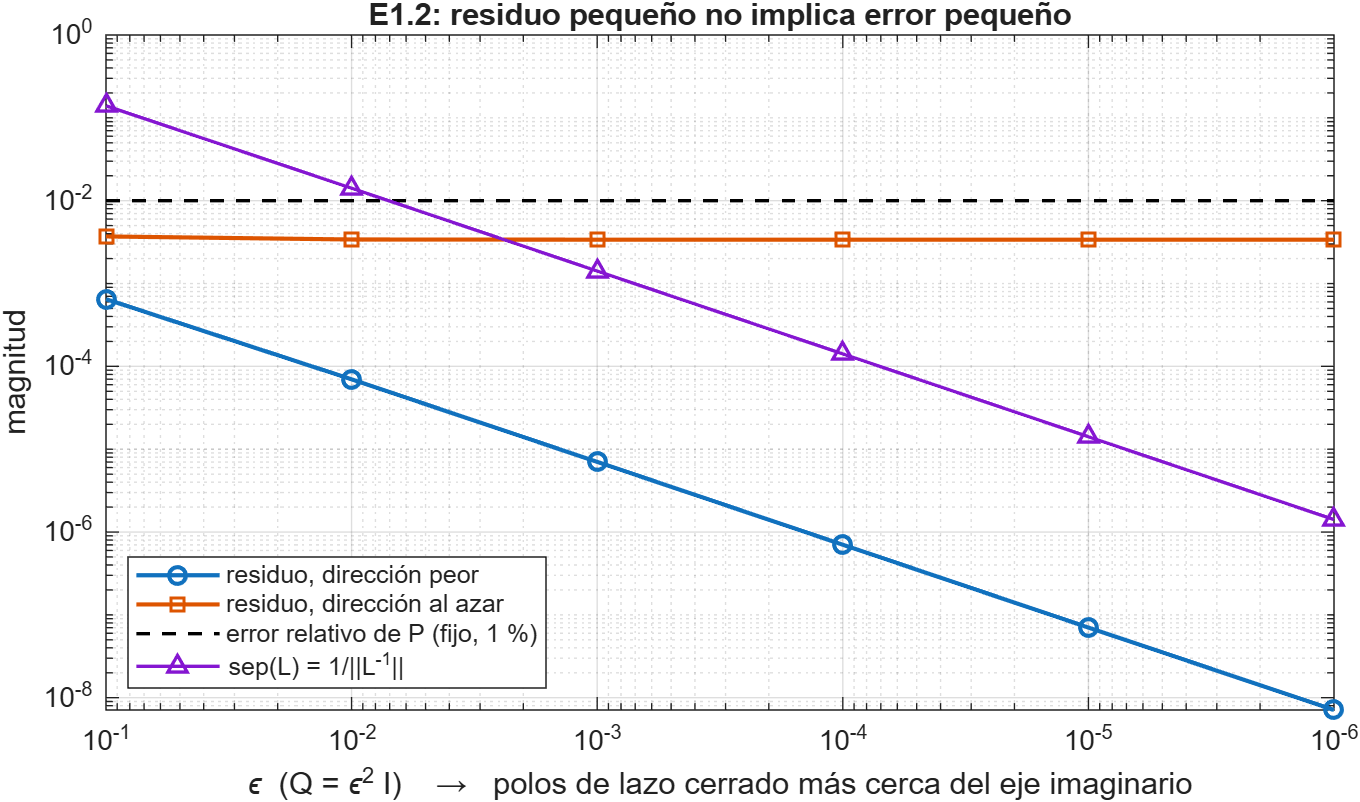
\includegraphics[width=0.74\linewidth]{E1_2_residuo_vs_error.png}
\caption{E1.2: con un error de $P$ fijo en $1\,\%$, el residuo en la dirección peor cae proporcional a
$\varepsilon$ junto con $\operatorname{sep}(\mathcal L)=1/\|\mathcal L^{-1}\|$; en una dirección aleatoria refleja el error.}\label{fig:e12}
\end{figure}

\paragraph{Interpretación.} El residuo es un error inverso: certifica el error directo solo multiplicado por
$\|\mathcal L^{-1}\|$, que actúa como número de condición \cite{higham2002,sun1998}. En el péndulo ese factor es
moderado y un residuo de $10^{-13}$ sí garantiza al menos nueve cifras correctas; en un lazo cerrado con polos
cerca del eje imaginario no, y entonces hay que verificar con una referencia independiente, como se hace en
E1.3.

\subsection{E1.3 --- Estudio de estrés numérico}
\paragraph{Planteamiento.} Tres familias de $13$ problemas, cada una con un solo parámetro: F1, $R=\rho R_0$ con
$\rho\in[10^{-8},10^4]$; F2, unidades de las velocidades, $T=\operatorname{diag}(1,1,s,s)$ con $s\in[10^{-6},10^6]$; y F3,
$Q_{11}=fQ_{0,11}$ con $f\in[10^{-12},1]$, que acerca los autovalores de $H$ al eje imaginario. Referencia:
Newton--Kleinman en aritmética de 40 dígitos (\texttt{vpa}) con los datos convertidos exactamente
(\texttt{sym(X,'f')}); su última corrección es $\le\V{e13_ref_correccion}$.

\paragraph{Desarrollo.} Se midió el error directo de los tres métodos, de \texttt{icare} y de variantes que aíslan
causas: con y sin equilibrado de $H$, con $P$ simetrizada, el haz extendido propio
(\texttt{src/riccati\_pencil.m}) sin escalado y con los vectores de escalado que elige \texttt{icare}
(\texttt{info.Sx}, \texttt{info.Sr}), y escalados propios ingenuos.

\paragraph{Resultados.} Sin equilibrado, Schur pierde $\V{e13_F1_cifras}$ cifras con $R=10^{-8}$ ($\V{e13_P3_schur}$) y
$\V{e13_F2_cifras}$ con $s=10^6$ ($\V{e13_F2_schur_smax}$), mientras que los vectores propios dan $\V{e13_P3_ham}$ en el
primer caso (figura \ref{fig:e13}). La predicción E1-P3 (anexo \ref{sec:pred}) esperaba lo contrario. El experimento
$2\times2$ \{vectores propios, Schur\} $\times$ \{con, sin equilibrado\} resolvió la discrepancia: \texttt{eig}
equilibra $H$ por defecto y \texttt{schur} no, y con el mismo tratamiento ambos métodos dan errores del mismo
orden en las $\V{e13_n_problemas}$ filas. El equilibrado recupera F2 (peor caso $\V{e13b_F2_bal_peor}$) pero no F1,
donde deja $\V{e13b_F1_hambal_Rmin}$: el daño ocurre al formar $S=BR^{-1}B^\top$, que mezcla escalas de $10^{8}$.
El haz extendido evita formar $S$ \cite{vandooren1981,arnold1984}; sin escalado aún pierde precisión
(peor caso F3 $\V{e13e_F3_haz_max}$, el mismo que \texttt{icare} sin escalado, $\V{e13e_F3_nosc_max}$), y con los
vectores de escalado de \texttt{icare} alcanza su precisión: peor caso $\V{e13e_F1_hazSx_peor}$,
$\V{e13e_F2_hazSx_peor}$ y $\V{e13e_F3_hazSx_peor}$ en F1, F2 y F3, frente a $\V{e13e_F1_icare_peor}$,
$\V{e13e_F2_icare_peor}$ y $\V{e13e_F3_icare_peor}$ de \texttt{icare} (figura \ref{fig:e13e}).

\begin{figure}[h]
\centering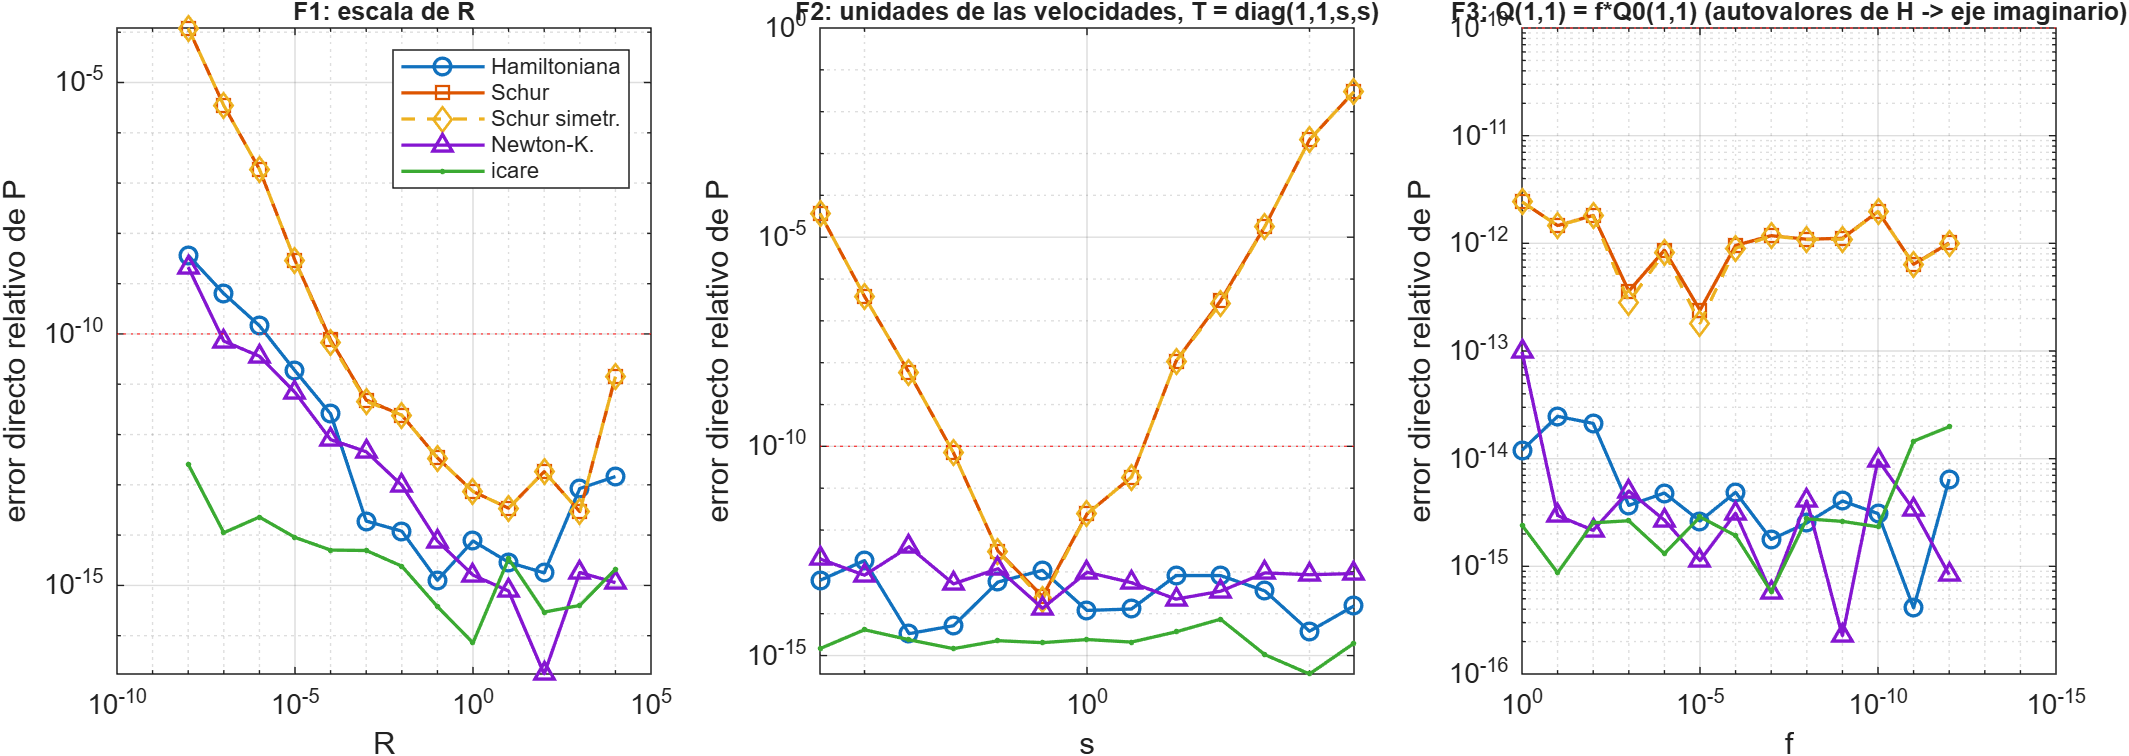
\includegraphics[width=\linewidth]{E1_3_estres.png}
\caption{E1.3: error directo frente a la referencia de 40 dígitos en las tres familias (sin equilibrado en los
métodos propios).}\label{fig:e13}
\end{figure}

\begin{figure}[h]
\centering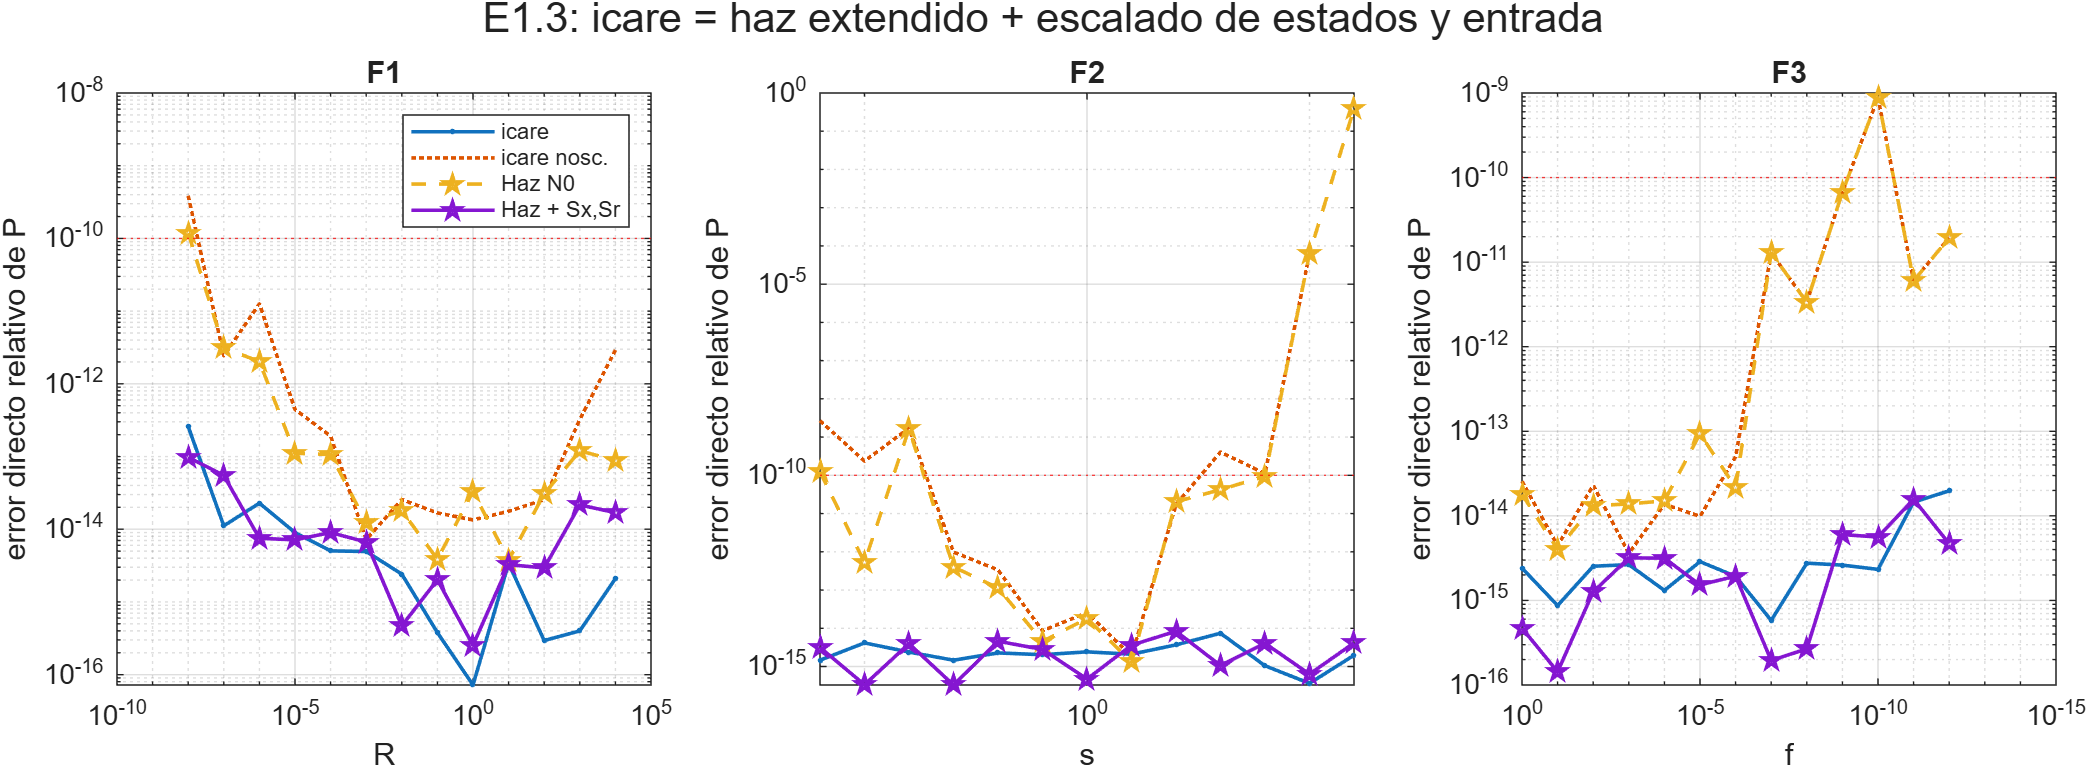
\includegraphics[width=\linewidth]{E1_3_icare_escalado.png}
\caption{E1.3: el haz extendido propio con los vectores de escalado de \texttt{icare} reproduce su precisión;
sin escalado (propio o \texttt{icare(\ldots,'noscaling')}) la pierde.}\label{fig:e13e}
\end{figure}

\paragraph{Verificación.} Se descartaron dos hipótesis: simetrizar $P$ no cambia el error y
$\operatorname{cond}(U_{11})$ vale solo $\V{e13_condU11_peor}$ en el peor caso. Los escalados ingenuos empeoran:
igualar $\|S\|$ y $\|Q\|$ ignora $A$ ($\V{e13d_F1_N3_peor}$ en F1) y \texttt{balance(A)} degenera porque la primera
columna de $A$ es nula, con $D=\operatorname{diag}(1,\V{e13e_D6_2},1,1)$. En F3 el error global sigue
$\le\V{e13_F3_max}$, pero el de la entrada pequeña $P_{11}$ llega a $\V{e13b_P11_nk_max}$ con Newton--Kleinman y a
$\V{e13b_P11_schur_max}$ con Schur sin equilibrado: la norma de Frobenius oculta el error de las entradas pequeñas.
Frente a la referencia, Newton--Kleinman confirma la convergencia cuadrática:
$e_k/e_{k-1}^2=\V{e13_nk_cociente6}$, $\V{e13_nk_cociente7}$ y $\V{e13_nk_cociente8}$ en las iteraciones 6 a 8.

\paragraph{Interpretación.} Un método de subespacio deja de ser confiable cuando los datos tienen escalas muy
distintas ($R$ muy pequeña o unidades incompatibles), no por el algoritmo de descomposición. Para esta planta
la solución confiable es el haz extendido con escalado de estados y entrada (\texttt{icare}). Newton--Kleinman
sin escalado también se degrada con $R=10^{-8}$ (error $\V{e13_nk_F1_max}$): sirve para refinar una solución ya
bien escalada, no para sustituir el escalado.

\subsection{E1.4 --- Frente de Pareto}
\paragraph{Planteamiento.} Con $Q=\operatorname{diag}(r_\theta(\pi/4)^{-2},r_\alpha(\pi/36)^{-2},0,0)$ y $R=R_0$, se generaron
$\V{e14_N}$ diseños con $r_\theta,r_\alpha\in[10^{-3},10^3]$ (malla logarítmica de $25\times25$). Cada diseño se
evalúa con tres objetivos cuadráticos esperados para una condición inicial aleatoria con covarianza declarada
$X_0=\operatorname{diag}(0.1^2,0.05^2,0.5^2,0.5^2)$:
\begin{equation}
J_i=\operatorname{tr}(C_iYC_i^\top),\qquad A_cY+YA_c^\top+X_0=0,\qquad C_\theta=e_1^\top,\;C_\alpha=e_2^\top,\;C_u=K,
\end{equation}
normalizados por $(\pi/4)^2$, $(\pi/36)^2$ y $V_{\max}^2=10^2$.

\paragraph{Resultados.} Los $\V{e14_N}$ diseños son estables ($\V{e14_n_estables}$) y no dominados
($\V{e14_n_nd}$), como predice la teoría para pesos positivos \cite{marler2004}, y cubren
$J_\theta/(\pi/4)^2\in[\V{e14_Jth_min},\V{e14_Jth_max}]$, $J_\alpha/(\pi/36)^2\in[\V{e14_Jal_min},\V{e14_Jal_max}]$ y
$J_u/10^2\in[\V{e14_Ju_min},\V{e14_Ju_max}]$ (figura \ref{fig:e14}). En la planta no lineal (simulador del kit),
$\V{e14_ok_C1}$ tienen éxito en C1, pero en C2 solo $\V{e14_ok_C2_ideal}$ con estado real y $\V{e14_ok_C2_real}$
con estimador, cuantización y ruido; $\V{e14_ok_C2_real_sat}$ cumplen además una fracción saturada $\le5\,\%$.

\paragraph{Verificación.} Los objetivos se calcularon por dos caminos, el gramiano (\texttt{sylvester}) y una
ecuación de Lyapunov dual por objetivo (\texttt{lyap\_kron}), con diferencia $\le\V{e14_dif_lyap}$; la suma ponderada
coincide con $\operatorname{tr}(PX_0)$ del LQR ($\le\V{e14_dif_suma}$); la integración con \texttt{ode45} de
$\V{e14_n_ode}$ diseños reproduce los objetivos ($\le\V{e14_dif_ode}$); y el diseño base reproduce los valores de
referencia del kit, $\max|u_c|=\V{e14_base_C1_uc}$~V en C1 y $\max|\theta|=\V{e14_base_C2_th}$~rad en C2. La
correlación de rangos de Spearman entre $J_u$ y $\max|u_c|$ en C1 es $\V{e14_spearman}$.

\begin{figure}[h]
\centering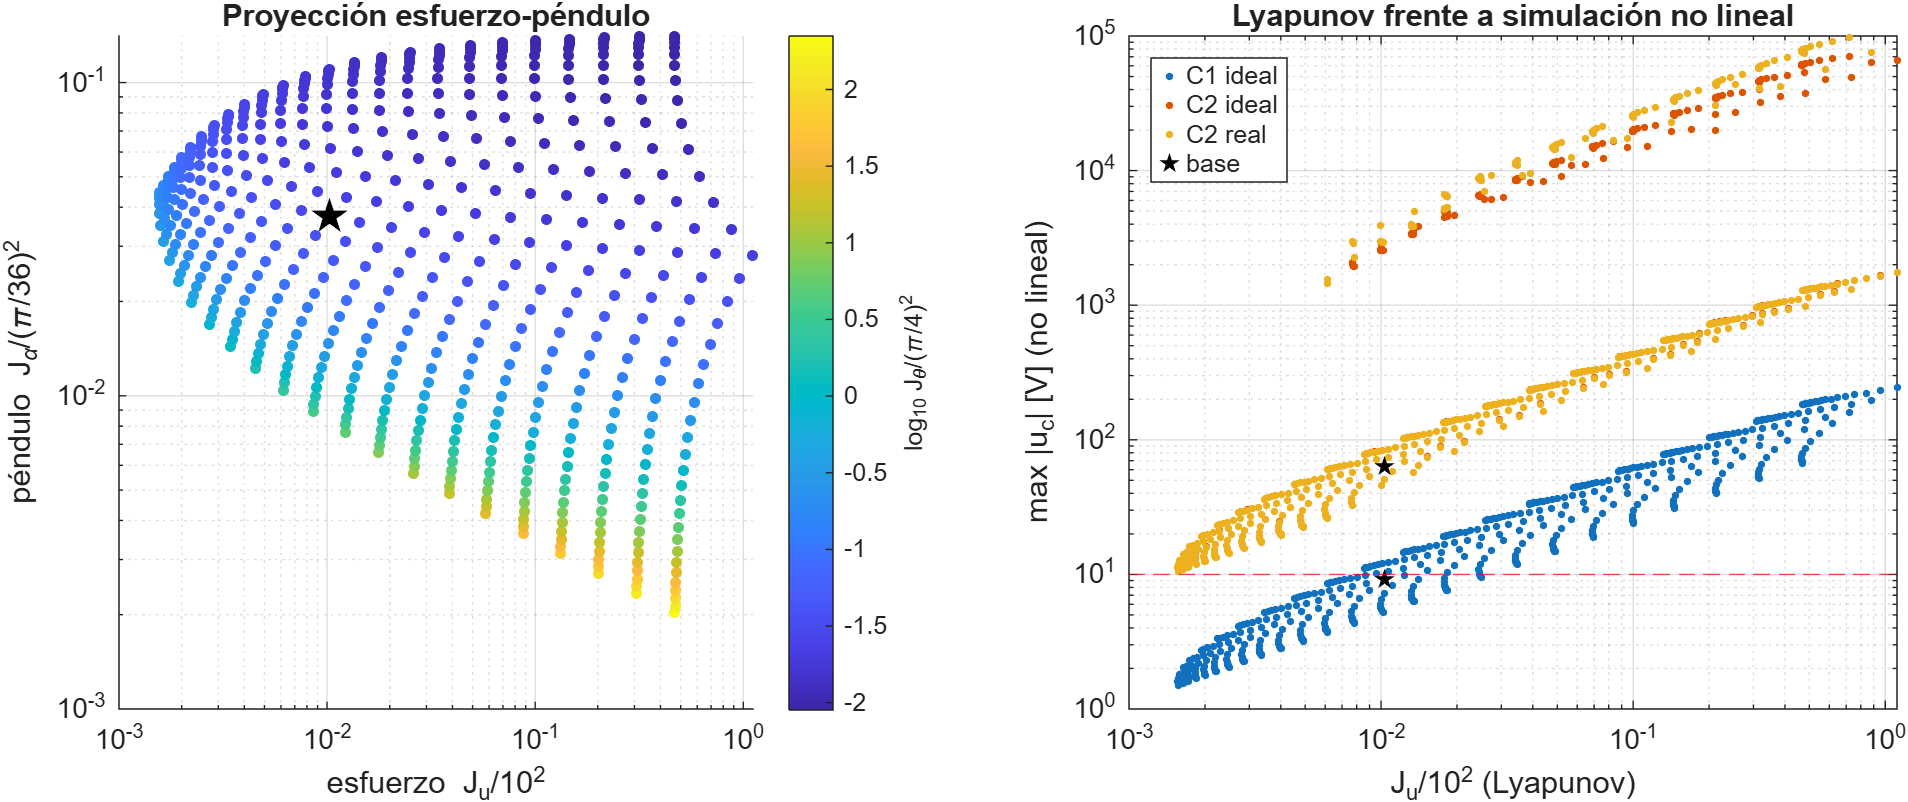
\includegraphics[width=\linewidth]{E1_4_proyecciones.png}
\caption{E1.4: proyección esfuerzo--péndulo del frente (color: $J_\theta$) y esfuerzo de Lyapunov frente al
$\max|u_c|$ simulado; la estrella es el diseño base.}\label{fig:e14}
\end{figure}

\paragraph{Interpretación.} El frente lineal ordena bien el esfuerzo (la correlación de rangos es alta), pero
no ve la saturación ni el sensor: la factibilidad en C2 se decide en la planta no lineal. $\V{e14_sensor_falla}$
diseños que se recuperan con estado real fallan con el estimador;
con una sola semilla de ruido, los $\V{e14_cambian}$ diseños que cambian de resultado deben leerse como frontera
difusa, no como clasificación exacta.

\subsection{E1.5 --- Optimización de los pesos con restricciones}
\paragraph{Planteamiento.} Problema de dos niveles: el nivel interior calcula el LQR para
$Q=\operatorname{diag}(r_\theta(\pi/4)^{-2},r_\alpha(\pi/36)^{-2},r_{\dot\theta},r_{\dot\alpha})$ y $R_0$; el exterior minimiza el costo
oficial del anexo B de la guía, promediado sobre los escenarios y referido al diseño base,
$J_{rel}=\tfrac14\sum_{c\in\{C1,C2,C3,C3b\}}J_c(K)/J_c(K_0)$, sujeto a: (R1) decaimiento
$\sigma=-\max\operatorname{Re}\lambda(A-BK)\ge\sigma_{\min}$; (R2) amortiguamiento $\zeta\ge0.5$; (R3) en C2,
$|\theta|\le\pi/2$ todo el ensayo y fracción saturada $\le5\,\%$; (R4) éxito en C1--C3b. La especificación del grupo
pide que $|\alpha|$ baje de 0.05 a 0.02~rad en unos 2~s, de donde $\sigma_{\min}=\ln(0.05/0.02)/2=\V{e15_sigma_min}$~s$^{-1}$.

\paragraph{Desarrollo.} De los $\V{e14_N}$ diseños de E1.4, $\V{e15_malla_R1R4}$ cumplen R1--R4. Dos búsquedas
\texttt{fminsearch} sobre los cuatro pesos (con penalización de las violaciones), desde el diseño base y desde el mejor
de la malla, llegan al mismo diseño ($J_{rel}=\V{e15_fmin_desde_base}$ y $\V{e15_fmin_desde_malla}$), pero con la
semilla 1. En 20 semillas su mejora se reduce a $J_{rel}=\V{e15_val_Jrel}\pm\V{e15_val_Jrel_desv}$ frente a
$\V{e15_Jrel_semilla1}$: el óptimo de una sola realización está sesgado \cite{smith2006}. Se reformuló como SAA
\cite{kleywegt2002}: costo promedio en las semillas 1--5 sobre una malla de $\V{e15b_n_malla}$ diseños y validación del ganador
en las semillas independientes 101--120 con una prueba $t$ pareada (19 grados de libertad, $t_{crit}=2.093$).

\paragraph{Resultados.} El óptimo SAA ($r_\theta=\V{e15b_r_th}$, $r_\alpha=\V{e15b_r_al}$) da, en validación,
$J_{rel}=\V{e15b_saa_Jrel}\pm\V{e15b_saa_Jrel_desv}$ con $t=\V{e15b_saa_t}$: no es significativamente mejor que el base.
Sí hay un compromiso significativo entre escenarios: mejora C2 en $\V{e15b_saa_mej_C2}\,\%$ ($t=\V{e15b_saa_t_C2}$) y
empeora C1 en $\V{e15b_saa_mej_C1}\,\%$ ($t=\V{e15b_saa_t_C1}$). Por la regla del grupo (cambiar el diseño solo con
mejora significativa en semillas independientes) se adopta $K_0$, que es factible: $\sigma=\V{e15d_base_sigma}$,
$\zeta=\V{e15d_base_zeta}$, $\V{esc_C2_sat}\,\%$ del tiempo saturado y $\max|\theta|=\V{esc_C2_th}$~rad en C2.

\paragraph{Verificación.} El piso de ruido del costo oficial explica parte de la dispersión: perturbar $K_0$ en
$10^{-15}$ cambia $J$ en $\V{e15c_piso_C1}\,\%$ (C1) y $\V{e15c_piso_C3}\,\%$ (C3) con cuantización, y como máximo en
$\V{e15c_piso_ideal_max}$ sin ella, porque una cuenta del encoder puede cambiar en algún instante. R1 es
coherente con la simulación: el tiempo de establecimiento en C1 es $\le\V{e15_ts_C1_max}$~s en las 20 semillas.
La predicción E1-P2 (más $R$ para cumplir C2) resultó opuesta: con $R\ge\V{e15_P2_m_falla}R_0$
($K_2\le\V{e15_P2_K2_falla}$~V/rad) el brazo supera $\pi/2$.

\paragraph{Bonificación: regiones de polos por LMI.} Con $X=P^{-1}$, $Y=KX$ y $M=AX-BY$, el LQR se escribe como
$\min\operatorname{tr}(Z)$ sujeto a la LMI de costo garantizado y
$\left[\begin{smallmatrix}Z&X_0^{1/2}\\X_0^{1/2}&X\end{smallmatrix}\right]\succ0$ \cite{boyd1994}; la región se impone con la misma
$X$: $M+M^\top+2\sigma X\prec0$ y
$\left[\begin{smallmatrix}\sin\phi(M+M^\top)&\cos\phi(M-M^\top)\\\cos\phi(M^\top-M)&\sin\phi(M+M^\top)\end{smallmatrix}\right]\prec0$,
$\phi=\arccos\zeta_{\min}$ \cite{chilali1996}. Sin región reproduce el LQR ($\|K-K_0\|/\|K_0\|=\V{e15d_K_lmi_vs_K0}$). Con la
región del grupo cuesta $+\V{e15d_costo_region}\,\%$ en $J_0$ aunque $K_0$ ya está dentro (logra
$\sigma=\V{e15d_sigma_g}$, $\zeta=\V{e15d_zeta_g}$): la matriz de Lyapunov común es conservadora. Frente al ajuste de
los pesos de posición de $Q$, el LQR es más barato al exigir decaimiento ($\sigma\ge4$: $\V{e15d_s4_Q}$ frente a
$\V{e15d_s4_LMI}$ veces $J_{0,base}$) y la LMI al exigir amortiguamiento ($\zeta\ge0.85$: $\V{e15d_z85_LMI}$ frente a
$\V{e15d_z85_Q}$) (figura \ref{fig:e15}). En validación no lineal el diseño LMI no mejora a $K_0$
($J_{rel}=\V{e15d_val_Jrel}\pm\V{e15d_val_Jrel_desv}$, $t=\V{e15d_val_t}$), y la región $\sigma\ge4$, alcanzable en el modelo
lineal, falla C2 incluso con estado real ($\V{e15d_s4_C2_sat_ideal}\,\%$ del tiempo saturado).

\begin{figure}[h]
\centering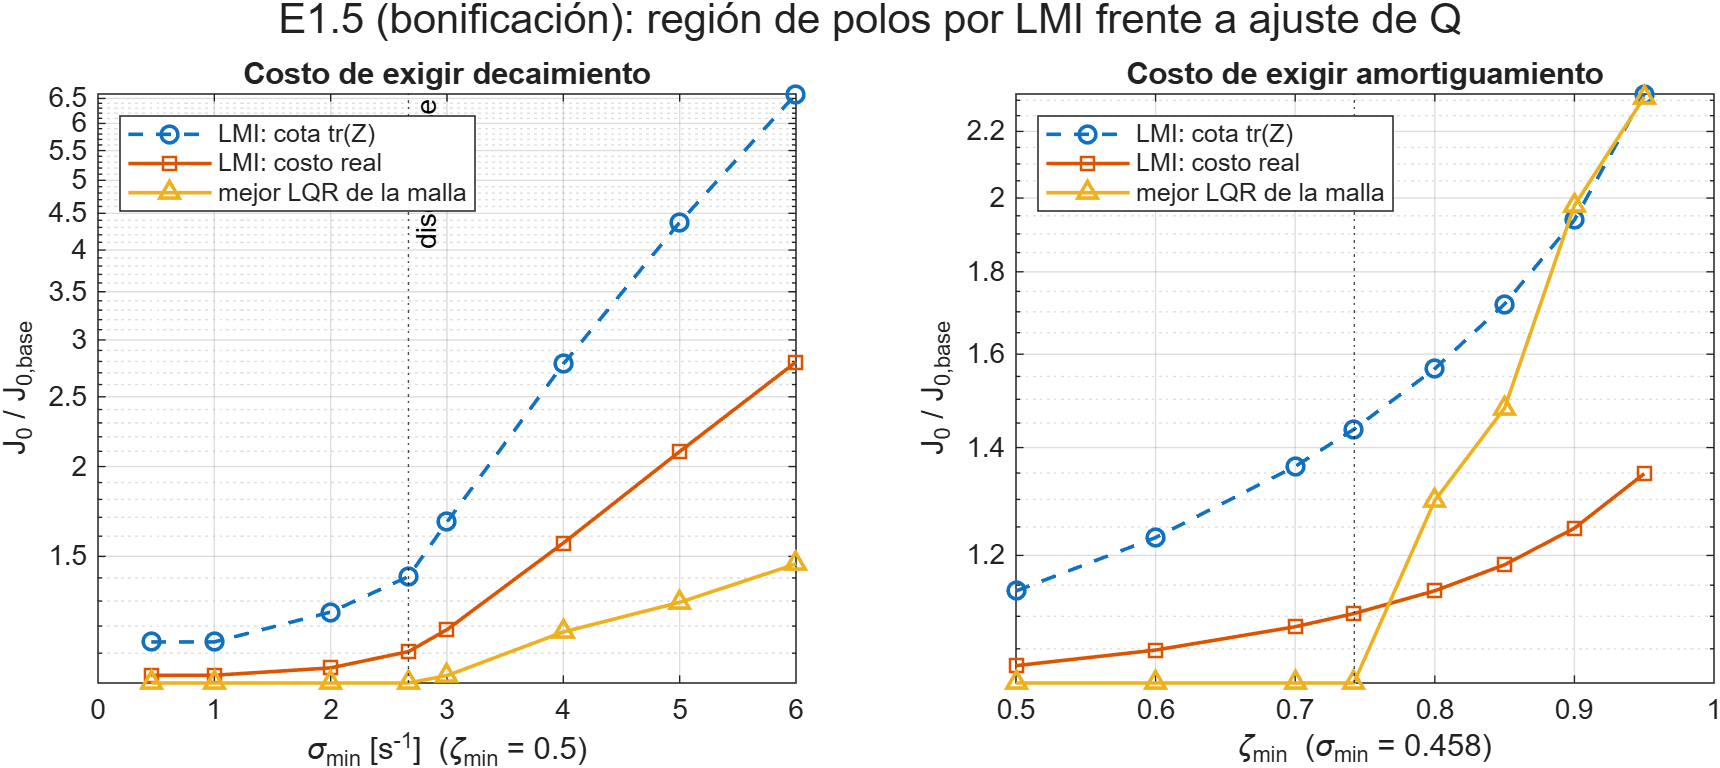
\includegraphics[width=\linewidth]{E1_5_lmi.png}
\caption{E1.5 (bonificación): costo $J_0/J_{0,base}$ de imponer la región por LMI (cota y costo real) y del mejor
LQR de la malla de E1.4 que cae en la región, en función de $\sigma_{\min}$ y de $\zeta_{\min}$.}\label{fig:e15}
\end{figure}

\paragraph{Interpretación.} Las especificaciones lineales (R1, R2) son fáciles de cumplir; las que restringen
el diseño son las no lineales de C2, y solo se pueden verificar simulando. Con un costo evaluado en un
simulador con cuantización y ruido, la mejora que reporta una optimización con una sola semilla es en buena parte
ruido; la decisión necesita validación independiente. Para esta planta, el diseño base ya está en la zona útil
del frente: lo que se gana en C2 se pierde en C1.

\subsection{E1.6 --- Región de atracción del regulador saturado}\label{sec:e16}
\paragraph{Planteamiento.} (a) Certificado: con $V(x)=x^\top Px$, el mayor $\rho$ tal que $|Kx|\le V_{\max}$ en
$\mathcal E=\{x^\top Px\le\rho\}$ es
\begin{equation}
\rho^\star=\frac{V_{\max}^2}{KP^{-1}K^\top}.
\end{equation}
Dentro de $\mathcal E$ el actuador no satura, $\dot V=-x^\top(Q_0+K^\top R_0K)x\le0$ y $\mathcal E$ es invariante; como
$(A,Q_0^{1/2})$ es observable, LaSalle \cite{lasalle1960} da convergencia al origen \cite{hu2001}. Hipótesis: modelo
lineal, tiempo continuo, estado exacto y sin límite de recorrido. (b) Estimación: Monte Carlo sobre la planta no
lineal saturada con lazo digital, $\V{e16_mc_N}$ condiciones iniciales uniformes en la caja
$|\theta|\le\pi/2$, $|\alpha|\le0.8$~rad, $|\dot\theta|,|\dot\alpha|\le10$~rad/s, cortes 2D de $81\times81$ y bisección radial
en $\V{e16_n_dir}$ direcciones aleatorias. ``Recuperado'': $|\alpha|<0.02$~rad y $|\dot\alpha|<0.2$~rad/s al cabo de 5~s;
``éxito'': además $|\theta|\le\pi/2$ en todo el ensayo.

\paragraph{Resultados.} $\rho^\star=\V{e16_rho}$; el elipsoide llega a $\V{e16_corte_alpha}$~rad sobre el eje $\alpha$ y a
$\V{e16_corte_theta}$~rad sobre $\theta$. La planta no lineal se recupera desde $\alpha_0=\V{e16_al_emp}$~rad con estado
real y cumple además $|\theta|\le\pi/2$ hasta $\V{e16_rad_ideal_exito}$~rad; con estimador, cuantización y ruido
(simulador oficial, 5 semillas), hasta $\V{e16_rad_oficial_exito}$~rad ($\V{e16_efecto_sensor}\,\%$). En la caja se
recupera el $\V{e16_mc_rec}\,\%$ de las condiciones ($\V{e16_mc_exito}\,\%$ con éxito). El certificado subestima el radio
entre $\V{e16_razon_min}$ y $\V{e16_razon_max}$ veces (mediana $\V{e16_razon_med}$; figura \ref{fig:e16}).

\begin{figure}[h]
\centering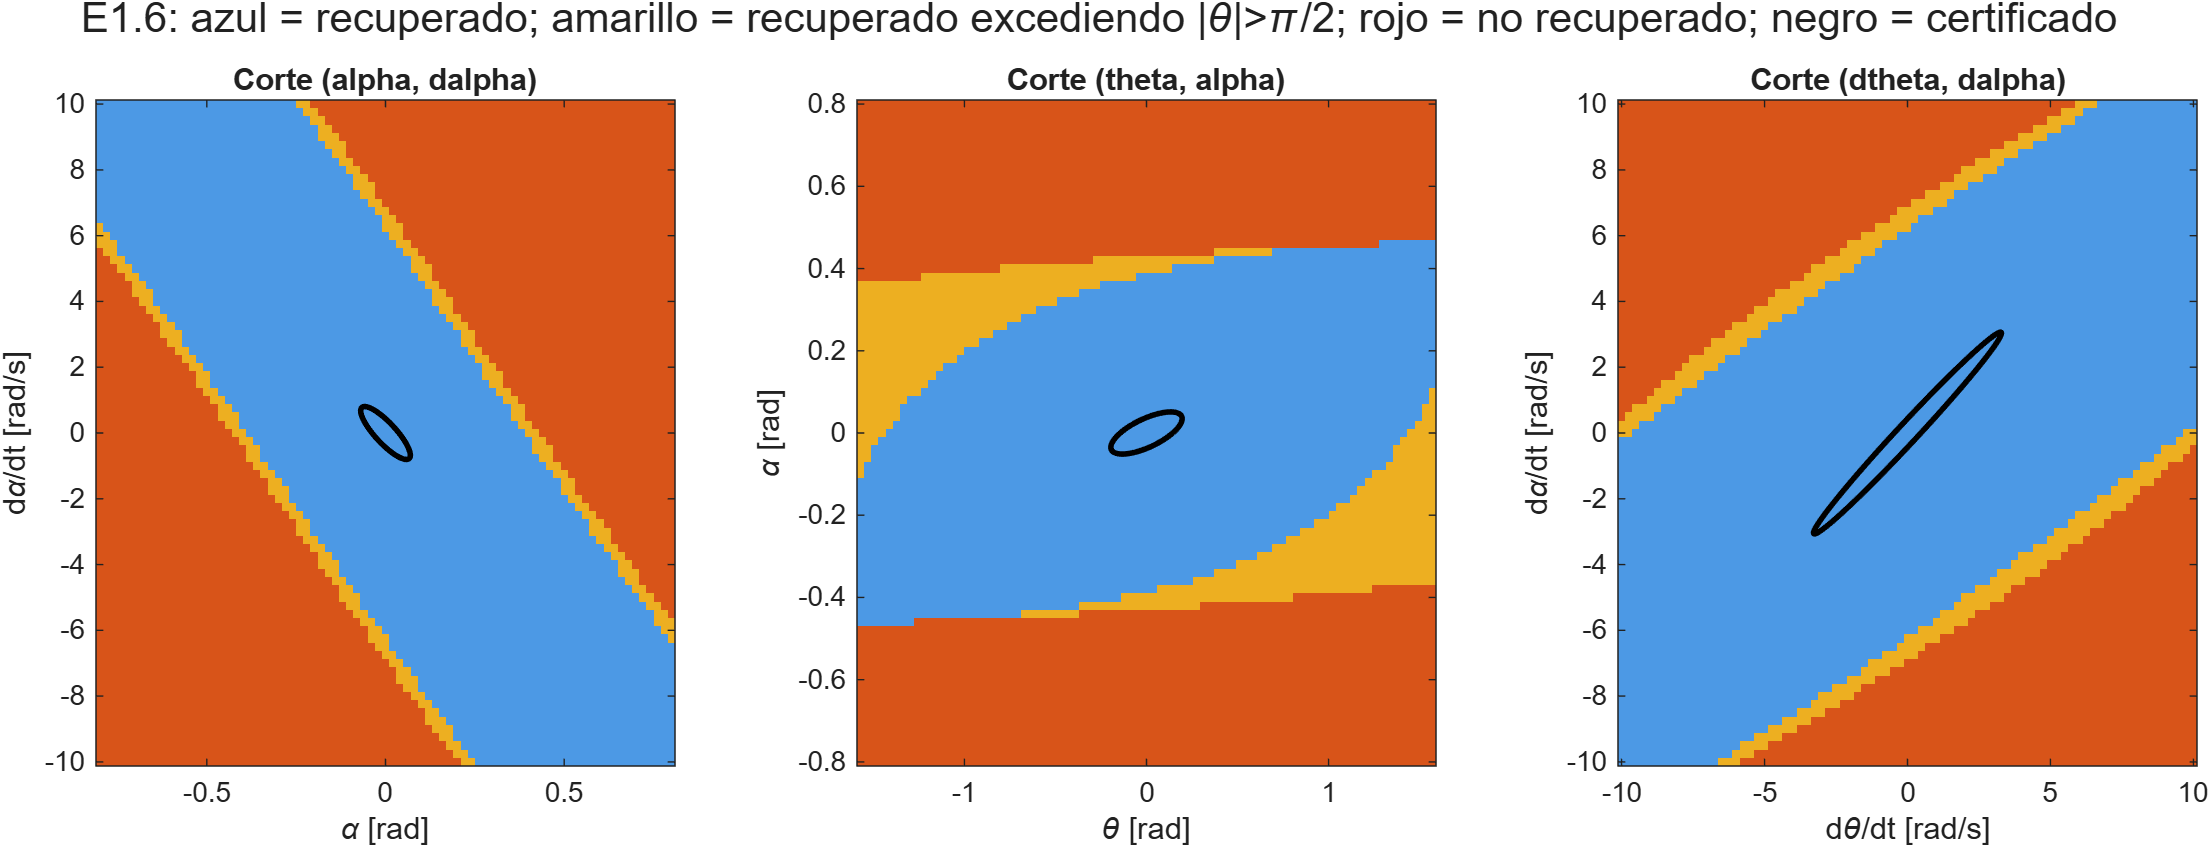
\includegraphics[width=\linewidth]{E1_6_cortes.png}
\caption{E1.6: cortes 2D de la región de atracción estimada (planta no lineal saturada) con el corte del
elipsoide certificado superpuesto.}\label{fig:e16}
\end{figure}

\paragraph{Verificación.} En $10^5$ puntos de la frontera de $\mathcal E$, $\max|Kx|=\V{e16_max_Kx}$~V; $\dot V<0$ en el
$\V{e16_dV_neg}\,\%$ de esos puntos también con la dinámica no lineal; el rango de la matriz de observabilidad de
$(A,Q_0^{1/2})$ es $\V{e16_rango_obs}$. De $\V{e16_in_n}$ condiciones sorteadas dentro de $\mathcal E$ se recuperan
$\V{e16_in_rec}$ en la planta no lineal muestreada, con $\max|u_c|=\V{e16_in_max_uc}$~V y $\V{e16_in_sat}$ muestras
saturadas. El simulador por lotes coincide con \texttt{simular\_qube} en $\V{e16_lote_coinc}$ de $\V{e16_lote_n}$
condiciones (diferencia final $\le\V{e16_lote_dif}$).

\paragraph{Interpretación.} Lo certificado es una garantía matemática para el modelo lineal; lo estimado es
evidencia numérica sobre la planta no lineal y depende de la caja, del horizonte y del criterio. La diferencia de
un orden de magnitud tiene dos causas: el certificado prohíbe toda saturación, mientras que la planta tolera
saturaciones breves, y se limita a un conjunto de nivel de una función cuadrática. Para el diseño final, C2
($\alpha_0=0.35$~rad) queda dentro de la región estimada con éxito, a solo $\V{e16_C2_margen}$~rad del borde, y
fuera del certificado: su recuperación es un hecho verificado por simulación, no garantizado.

% =====================================================================
\section{Escenarios C1--C5}
Diseño final: $K_0$ (sección E1.5). Simulador oficial del kit con saturación, estimador base, cuantización y
ruido base (semilla 1 en C1--C3b; en C4, planta $i$ con semilla $1000+i$ y ruido con semilla $i$). Tabla generada
desde \texttt{results.json}.

% Generado automáticamente por generar_results.m desde results.json. No editar a mano.
\begin{center}\small\setlength{\tabcolsep}{3.5pt}
\begin{tabular}{@{}l l r r r r r r@{}}
\toprule
Escenario & Estado & $J$ & $t_s$ [s] & $\max|u_c|$ [V] & $\max|u|$ [V] & Saturado [\%] & $\max|\theta|$ [rad] \\
\midrule
C1 & ok & 0.0331 & 0.114 & 8.96 & 8.96 & 0.0 & 0.109 \\
C2 & ok & 3.3267 & 1.136 & 63.82 & 10.00 & 1.9 & 1.345 \\
C3 & ok & 0.0185 & 0.050 & 5.56 & 5.56 & 0.0 & 0.036 \\
C3b & ok & 0.2970 & 0.416 & 26.50 & 10.00 & 1.1 & 0.248 \\
\midrule
C4 & 200 de 200 & 0.0349 $\pm$ 0.0035 & 0.180 (p95) & 8.96 & -- & -- & 0.131 (p95) \\
C5 & no\_aplica & \multicolumn{6}{l}{(solo se exige a E4)} \\
\bottomrule
\end{tabular}
\end{center}


El diseño cumple los cuatro escenarios. En C1 se establece en $\V{esc_C1_ts}$~s, muy por debajo de los 2~s
de la especificación; en C2 el mando calculado llega a $\V{esc_C2_uc}$~V, pero el actuador satura solo el
$\V{esc_C2_sat}\,\%$ del tiempo y el brazo no pasa de $\V{esc_C2_th}$~rad; en C3b el impulso grande satura el
$\V{esc_C3b_sat}\,\%$ del tiempo sin comprometer el éxito. En C4, $\V{esc_C4_exito}$ de $\V{esc_C4_n}$ plantas con
$\pm20\,\%$ en $m_p$, $L_p$, $R_m$ y $k_t$ tienen éxito, con $J=\V{esc_C4_J}\pm\V{esc_C4_J_desv}$ y percentil 95 de
$\max|\theta|$ de $\V{esc_C4_th_p95}$~rad. C5 solo se exige a E4. Videos de C1 y C2 en \texttt{videos/}.

% =====================================================================
\section{Conclusiones}
\begin{itemize}
\item \textbf{Qué método es confiable.} Para el diseño base los tres métodos dan la misma $P$ dentro de
$\V{e11_difmax_base}$ y pasan las cuatro pruebas de E1.2. Con datos mal escalados, el método confiable es el haz
extendido con escalado de estados y entrada (\texttt{icare}): error $\le\V{e13e_hazSx_peor}$ en los
$\V{e13_n_problemas}$ problemas de estrés. Newton--Kleinman, con ganancia inicial estabilizante, sirve como
refinamiento de una solución bien escalada y converge de forma cuadrática.
\item \textbf{Cuándo deja de serlo.} Los métodos de subespacio fallan por el escalado y no por la
descomposición: sin equilibrado pierden hasta $\V{e13_F2_cifras}$ cifras, y formar $S$ con $R=10^{-8}$ cuesta precisión
incluso equilibrando. El residuo no basta para detectarlo cuando $\|\mathcal L^{-1}\|$ es grande, y el error en norma
de Frobenius oculta el de las entradas pequeñas de $P$.
\item \textbf{Cómo se traducen las especificaciones.} Decaimiento y amortiguamiento se traducen en restricciones
sobre los polos; saturación y recorrido, solo simulando la planta no lineal. Con validación en semillas
independientes, ningún LQR mejora de forma significativa al diseño base, que cumple todas las restricciones. La
garantía verificable sobre la planta saturada es local y conservadora (elipsoide de $\V{e16_corte_alpha}$~rad en
$\alpha$); la región real, $\V{e16_razon_med}$ veces mayor en mediana, es una estimación numérica.
\end{itemize}
\textbf{Límites de validez.} Modelo de varilla uniforme con amortiguamiento viscoso supuesto por el kit; el
certificado vale para el modelo lineal en tiempo continuo; las fracciones del Monte Carlo dependen de la caja y del
horizonte declarados; la optimización se limitó a LQR con $Q$ diagonal; y el costo oficial tiene un piso de ruido por
cuantización ($\V{e15c_piso_C1}\,\%$ en C1 y $\V{e15c_piso_C3}\,\%$ en C3), que limita la resolución de cualquier comparación entre diseños.

\bibliographystyle{plainnat}
{\small\bibliography{referencias}}

\clearpage
\appendix
% =====================================================================
% Fichas de evidencia del encargo E1 (sección 4.2 de la guía).
% Una ficha por inciso. Los números deben coincidir con results.json
% regenerado desde cero (se sincronizarán al cerrar el encargo).
% =====================================================================
\section{Fichas de evidencia}

% ---------------------------------------------------------------------
\begin{recuadro}[title=Ficha de evidencia — E1.1: tres métodos de solución de la ecuación de Riccati]
\begin{tabularx}{\linewidth}{@{}>{\bfseries}p{3.1cm} >{\raggedright\arraybackslash}X@{}}
Afirmación &
Los métodos (a) vectores propios de la Hamiltoniana, (b) Schur real ordenado y (c) Newton--Kleinman
resuelven la ecuación de Riccati del diseño base $(Q_0,R_0)$ con una diferencia máxima entre ellos de
$2.5\times10^{-12}$. En el banco de seis problemas, (a) y (c) quedan por debajo de $10^{-10}$ frente a
\texttt{icare} en todos los casos; (b) supera esa tolerancia solo en el modelo de 5 estados con armadura
($7.2\times10^{-9}$), cuya $P$ es casi singular ($\lambda_{\min}(P)=7.4\times10^{-14}$). \\[3pt]
Evidencia &
Tablas de \texttt{e1\_1\_metodos.m}; figura \texttt{figuras/E1\_1\_errores.png};
datos en \texttt{resultados/E1\_1.mat}. Implementación en \texttt{src/riccati\_hamiltoniano.m},
\texttt{src/riccati\_schur.m}, \texttt{src/riccati\_newton.m}. \\[3pt]
Comprobación independiente &
(1) Biblioteca: \texttt{icare}; diseño base: (a) $9.7\times10^{-15}$, (b) $2.4\times10^{-12}$,
(c) $1.0\times10^{-13}$.
(2) Kit: $P_0$ de \texttt{diseno\_base\_ref.json} (\texttt{pruebas\_E1.m}); $K$ de Newton frente a
$K_0$: $5.4\times10^{-14}$.
(3) Respuesta conocida: $\dot x=x+u$, $K=1+\sqrt{1+q}$; error $\le 2.2\times10^{-16}$ para
$q\in[10^{-6},1]$.
(4) Convergencia cuadrática de Newton--Kleinman: residuo
$1.7\times10^{-3}\to3.6\times10^{-5}\to1.2\times10^{-8}\to1.2\times10^{-15}$ (iteraciones 6 a 9). \\[3pt]
Supuestos &
$(A,B)$ estabilizable y $(A,Q^{1/2})$ detectable. Newton requiere una ganancia inicial
estabilizante: Bass con $\beta=20$ en 4 estados; en 5 estados Bass exigiría $\beta>7240$ y no
estabiliza numéricamente, por lo que se usa $[K_0\;0]$. El método (b) se implementó sin escalado
ni simetrización de $P$; con balanceo (como \texttt{icare}) su error debería disminuir, lo que
cambiaría la ordenación de los métodos.
\end{tabularx}
\end{recuadro}

% ---------------------------------------------------------------------
\begin{recuadro}[title=Ficha de evidencia — E1.2: verificación de las soluciones y condicionamiento]
\begin{tabularx}{\linewidth}{@{}>{\bfseries}p{3.1cm} >{\raggedright\arraybackslash}X@{}}
Afirmación &
Un residuo pequeño no implica un error pequeño en $P$: en el oscilador
$A=\left[\begin{smallmatrix}0&1\\-1&0\end{smallmatrix}\right]$, $Q=\varepsilon^2 I$, una $P$ con error relativo
de $1\,\%$ tiene residuo normalizado de solo $7.1\times10^{-9}$ para $\varepsilon=10^{-6}$, porque
$\|\mathcal{L}^{-1}\|_2=7.07\times10^{5}$, con $\mathcal{L}(X)=A_c^\top X+XA_c$. En el péndulo,
$\|\mathcal{L}^{-1}\|_2=86$ y la cota $\|\mathcal{L}^{-1}\|\,\|\mathrm{Res}\|/\|P\|\le 6.9\times10^{-10}$
acota el error real ($\le 2.4\times10^{-12}$). Las tres soluciones del péndulo pasan las cuatro
pruebas: residuo $\le1.4\times10^{-13}$, asimetría $\le1.9\times10^{-13}$,
$\lambda_{\min}(P)=3.4\times10^{-4}>0$ y $\max\operatorname{Re}\lambda(A-BK)=-2.668$. \\[3pt]
Evidencia &
Tablas de \texttt{e1\_2\_verificacion.m}; figura \texttt{figuras/E1\_2\_residuo\_vs\_error.png};
datos en \texttt{resultados/E1\_2.mat}; \texttt{src/operador\_lyapunov.m}, \texttt{src/verificar\_riccati.m}. \\[3pt]
Comprobación independiente &
(1) Solución analítica del oscilador: $p_2=\varepsilon^2/(1+\sqrt{1+\varepsilon^2})$,
$p_3=\sqrt{2p_2+\varepsilon^2}$, $p_1=p_3(1+p_2)$.
(2) Primer orden: $\mathrm{Res}(P^\star+\Delta)\approx\mathcal{L}(\Delta)$ con discrepancia de $0.7\,\%$ en
todas las filas (término cuadrático $\Delta S\Delta$).
(3) Control: en una dirección aleatoria el mismo error da residuo $3.4\times10^{-3}$.
(4) La propia \texttt{icare} pierde precisión frente a la solución exacta: de $1.8\times10^{-14}$
($\varepsilon=10^{-1}$) a $2.1\times10^{-6}$ ($\varepsilon=10^{-6}$). \\[3pt]
Supuestos &
Análisis de primer orden (válido si $\|\Delta S\Delta\|\ll\|\mathcal{L}(\Delta)\|$, aquí $0.7\,\%$).
La dirección ``peor'' es la del menor valor singular de $\mathcal{L}$ (caso pesimista); otra dirección
da un residuo mayor. La normalización del residuo es la de \texttt{residuo\_riccati.m}; otra
normalización cambia los valores, no la tendencia. $\|\mathcal{L}^{-1}\|$ no explica por completo el
error de \texttt{icare}, que crece más rápido; el condicionamiento completo de la ecuación de Riccati
(Kenney, Laub y Wette, 1990) incluye otros términos.
\end{tabularx}
\end{recuadro}

% ---------------------------------------------------------------------
\begin{recuadro}[title=Ficha de evidencia — E1.3: estudio de estrés numérico]
\begin{tabularx}{\linewidth}{@{}>{\bfseries}p{3.1cm} >{\raggedright\arraybackslash}X@{}}
Afirmación &
La precisión la decide el \emph{escalado de los datos}, no el método de subespacio. Sin balanceo,
vectores propios y Schur pierden hasta 12 cifras con $R=10^{-8}$ ($1.2\times10^{-4}$) y 14 con las
velocidades en otras unidades ($s=10^{6}$: $3.0\times10^{-2}$). Balancear $H$ recupera F2
($1.6\times10^{-14}$), pero en F1 deja $3.6\times10^{-9}$: formar $S=BR^{-1}B^\top$ ya mezcla escalas
incompatibles. \texttt{icare} evita ambos problemas: usa el haz extendido (no forma $S$) y escala
estados y entrada; reproducido con código propio, alcanza su precisión (peor caso $9.8\times10^{-14}$).
Con autovalores de $H$ cerca del eje imaginario, el error global sigue $\le2.4\times10^{-12}$, pero el
de la entrada pequeña $P_{11}$ llega a $2.6\times10^{-9}$. \\[3pt]
Evidencia &
\texttt{e1\_3\_estres.m} (tres familias, 39 problemas), \texttt{e1\_3b\_balanceo.m}, \texttt{e1\_3c\_icare.m},
\texttt{e1\_3d\_escalado.m}, \texttt{e1\_3e\_icare\_escalado.m}; figuras \texttt{E1\_3\_*.png}; datos en
\texttt{resultados/E1\_3*.mat}; \texttt{src/riccati\_pencil.m}, \texttt{src/escalar\_riccati.m}. \\[3pt]
Comprobación independiente &
(1) Referencia en precisión extendida: Newton--Kleinman con \texttt{vpa} de 40 dígitos y datos exactos
(\texttt{sym(X,'f')}).
(2) Experimento $2\times2$ \{vectores propios, Schur\} $\times$ \{con, sin balanceo\}: las columnas con el
mismo balanceo coinciden en las 39 filas.
(3) Haz extendido propio sin escalado frente a \texttt{icare(\ldots,'noscaling')}: F3 idénticos fila a fila
(p.\ ej.\ $8.8\times10^{-10}$ ambos), F2 $6.4\times10^{-5}$ frente a $6.3\times10^{-5}$ ($s=10^5$); con $s=10^6$
\texttt{icare} sin escalado no devuelve solución.
(4) El mismo haz con los vectores de escalado de \texttt{icare} (\texttt{info.Sx}, \texttt{info.Sr}):
peor caso F1/F2/F3 $9.8\times10^{-14}$, $8.4\times10^{-15}$, $1.6\times10^{-14}$, frente a \texttt{icare}
$2.6\times10^{-13}$, $7.4\times10^{-15}$, $2.0\times10^{-14}$.
(5) Hipótesis descartadas: simetrizar $P$ y $\operatorname{cond}(U_{11})$ (vale 4.0 en el peor caso).
(6) Newton--Kleinman cuadrático frente a \texttt{vpa}: $e_k/e_{k-1}^2=0.81,\,1.03,\,1.07$. \\[3pt]
Supuestos &
Se reutiliza el escalado que elige \texttt{icare}, no su regla de elección. Los escalados propios
ingenuos empeoran: igualar $\|S\|$ y $\|Q\|$ ignora $A$ ($5.3\times10^{-8}$ en F1), y \texttt{balance(A)}
degenera porque la primera columna de $A$ es nula ($\theta$ no aparece en la dinámica), con
$D=\operatorname{diag}(1,\,6\times10^{-8},\,1,\,1)$. El error en norma de Frobenius oculta el de entradas
pequeñas; por eso se reporta también el de $P_{11}$. Cada familia varía un solo parámetro.
\end{tabularx}
\end{recuadro}

% ---------------------------------------------------------------------
\begin{recuadro}[title=Ficha de evidencia — E1.4: frente de Pareto]
\begin{tabularx}{\linewidth}{@{}>{\bfseries}p{3.1cm} >{\raggedright\arraybackslash}X@{}}
Afirmación &
Los 625 diseños LQR obtenidos al escalar los pesos de brazo y péndulo entre $10^{-3}$ y $10^{3}$ (normalización
de Bryson del diseño base) son todos estables y no dominados, y forman una superficie de Pareto con
$J_\theta/(\pi/4)^2\in[8.96\times10^{-3},\,2.23\times10^{2}]$, $J_\alpha/(\pi/36)^2\in[2.03\times10^{-3},\,0.141]$ y
$J_u/10^2\in[1.56\times10^{-3},\,1.11]$. En la planta no lineal, los 625 tienen éxito en C1, pero en C2 solo
147 (estado real) y 115 (estimador base, cuantización y ruido); 101 cumplen además una fracción saturada
$\le5\,\%$. 48 diseños exitosos con estado real fallan con el sensor. \\[3pt]
Evidencia &
\texttt{e1\_4\_pareto.m}; figuras \texttt{figuras/E1\_4\_pareto3d.png} y \texttt{figuras/E1\_4\_proyecciones.png};
datos en \texttt{resultados/E1\_4.mat} y simulaciones en \texttt{resultados/E1\_4\_sim.mat}. \\[3pt]
Comprobación independiente &
(1) Lyapunov por dos caminos: primal (gramiano, \texttt{sylvester}) y dual (una ecuación por objetivo,
\texttt{lyap\_kron}): diferencia $\le1.3\times10^{-9}$.
(2) Respuesta conocida: la suma ponderada de los objetivos coincide con $\operatorname{tr}(PX_0)$ del LQR
($\le1.9\times10^{-10}$), y el filtro de Pareto declara no dominados 625 de 625, como predice la teoría.
(3) Simulación lineal con \texttt{ode45} en 10 diseños: diferencia $\le2.3\times10^{-11}$.
(4) \texttt{icare} frente a la Hamiltoniana balanceada: $\le8.9\times10^{-11}$.
(5) El diseño base reproduce $K_0$ y los valores del kit: 9.12~V y 1.237~rad (estado real), 63.82~V y
1.345~rad (con estimador).
(6) El esfuerzo de Lyapunov ordena el esfuerzo no lineal: correlación de rangos de Spearman 0.960 entre
$J_u$ y $\max|u_c|$ en C1. \\[3pt]
Supuestos &
Covarianza inicial declarada $X_0=\operatorname{diag}(0.1^2,\,0.05^2,\,0.5^2,\,0.5^2)$ (unidades SI): otra $X_0$
cambia la forma del frente, no la no dominancia. Los objetivos esperados son lineales y no ven la
saturación; por eso la factibilidad se juzga en la planta no lineal. C2 con sensor se simuló con una sola
semilla de ruido: los 64 diseños que cambian de resultado entre estado real y sensor están cerca del límite
y podrían cambiar con otra semilla. La malla varía dos pesos con $R$ fija; escalar $Q$ y $R$ a la vez no
cambia $K$.
\end{tabularx}
\end{recuadro}

% ---------------------------------------------------------------------
\begin{recuadro}[title=Ficha de evidencia — E1.5: optimización de los pesos con restricciones]
\begin{tabularx}{\linewidth}{@{}>{\bfseries}p{3.1cm} >{\raggedright\arraybackslash}X@{}}
Afirmación &
Con las restricciones del grupo (decaimiento $\sigma\ge0.458$~s$^{-1}$, amortiguamiento $\zeta\ge0.5$, C2 con
$|\theta|\le\pi/2$ y saturación $\le5\,\%$, éxito en C1--C3b), ningún LQR mejora de forma significativa el
costo oficial promedio del diseño base: el óptimo por promedio de 5 semillas ($r_\theta=1.58$, $r_\alpha=1$)
da $J_{rel}=0.9994\pm0.0225$ en 20 semillas independientes ($t=0.12$). Hay un compromiso significativo:
penalizar más el brazo mejora C2 ($+1.5\,\%$, $t=45.8$) y empeora C1 ($-1.2\,\%$, $t=-4.6$). El diseño base
es factible ($\sigma=2.668$, $\zeta=0.742$, saturación 1.9\,\%, $\max|\theta|=1.345$~rad en C2) y se adopta
como diseño final. \\[3pt]
Evidencia &
\texttt{e1\_5\_restricciones.m}, \texttt{e1\_5b\_saa.m}, \texttt{e1\_5c\_sensibilidad.m}, \texttt{src/diseno\_final.m};
figuras \texttt{figuras/E1\_5\_*.png}; datos en \texttt{resultados/E1\_5.mat} y \texttt{E1\_5b.mat}. \\[3pt]
Comprobación independiente &
(1) Validación con semillas 101--120, no usadas para elegir, en comparación pareada con el base (prueba
$t$, 19 grados de libertad).
(2) Dos búsquedas \texttt{fminsearch} desde puntos distintos llegan al mismo diseño ($J_{rel}=0.9625$ y
$0.9614$ con la semilla 1).
(3) Piso de ruido del costo oficial: perturbar $K_0$ en $10^{-15}$ cambia $J$ en 0.55\,\% (C1), 0.01\,\% (C2),
3.1\,\% (C3) y 0.09\,\% (C3b) con cuantización, y en $\sim10^{-16}$ sin ella; explica el $J_{rel}=0.9991$ del base
recalculado con \texttt{icare}.
(4) $\sigma\ge0.458$ es coherente con la simulación: tiempo de establecimiento en C1 $\le0.132$~s.
(5) La optimización con una sola semilla sobreestimó la mejora ($0.961$ frente a $0.9945\pm0.019$). \\[3pt]
Supuestos &
$J_{rel}$ pondera igual los cuatro escenarios: dar más peso a C2 y C3b favorecería un diseño más agresivo
(el óptimo de la semilla 1 mejora C3b en $5.2\,\%$, $t=8.3$, pero empeora C1 en $8.2\,\%$). Búsqueda en LQR con
$Q$ diagonal; los pesos de las velocidades no ayudaron (\texttt{fminsearch} los llevó al mínimo). $\sigma_{\min}$
proviene de una envolvente exponencial aproximada. La prueba $t$ supone diferencias aproximadamente normales.
\end{tabularx}
\end{recuadro}

% ---------------------------------------------------------------------
\begin{recuadro}[title=Ficha de evidencia — E1.5 (bonificación): síntesis por regiones de polos con LMI]
\begin{tabularx}{\linewidth}{@{}>{\bfseries}p{3.1cm} >{\raggedright\arraybackslash}X@{}}
Afirmación &
Imponer la región del grupo ($\sigma\ge0.458$, $\zeta\ge0.5$) por LMI con Lyapunov común cuesta $+2.5\,\%$ en
$J_0$ aunque $K_0$ ya está en la región: el método es conservador (logra $\sigma=2.939$, $\zeta=0.885$). Frente
al ajuste de los dos pesos de posición de $Q$, el ajuste de $Q$ es más barato al exigir decaimiento
($\sigma\ge4$: $1.18$ frente a $1.57$; $\sigma\ge6$: $1.46$ frente a $2.79$, en $J_0/J_{0,base}$) y la LMI lo es al
exigir amortiguamiento ($\zeta\ge0.85$: $1.18$ frente a $1.48$; $\zeta\ge0.9$: $1.25$ frente a $1.98$). Una región
alcanzable en el modelo lineal no garantiza la planta saturada: con $\sigma\ge4$ el diseño cumple C1 pero
falla C2 incluso con estado real ($99.9\,\%$ del tiempo saturado). \\[3pt]
Evidencia &
\texttt{e1\_5d\_lmi.m}, \texttt{src/lqr\_region\_lmi.m} (LMI Lab); figura \texttt{figuras/E1\_5\_lmi.png};
datos en \texttt{resultados/E1\_5\_lmi.mat}. \\[3pt]
Comprobación independiente &
(1) Respuesta conocida: sin región, la LMI reproduce el LQR ($\|K-K_0\|/\|K_0\|=1.3\times10^{-4}$, costo
$1.000000\,J_{0,base}$).
(2) Los polos de cada diseño, calculados con \texttt{eig}, cumplen la región pedida en los 16 casos.
(3) La cota $\operatorname{tr}(Z)$ queda por encima del costo real $J_0$ (Lyapunov propio) en todos los casos.
(4) Validación no lineal con semillas 101--120: el diseño LMI de la región del grupo cumple R3--R4 en
20 de 20, pero no mejora a $K_0$ ($J_{rel}=0.9982\pm0.0216$, $t=0.37$): mejora C3b ($+7.6\,\%$) y empeora C1
($-6.6\,\%$) y C2 ($-3.2\,\%$). \\[3pt]
Supuestos &
Una sola matriz de Lyapunov para el costo y la región (formulación de Chilali y Gahinet): la cota es
conservadora. La comparación con el ajuste de $Q$ usa solo los pesos de posición de la malla de E1.4; con
pesos en las velocidades el LQR podría amortiguar más barato. Con 5 semillas (1--5) el diseño LMI parecía
$2.3\,\%$ mejor ($0.977\pm0.009$); no se confirmó con 20 semillas independientes. Precisión del solucionador
LMI: $\sim10^{-4}$ en $K$.
\end{tabularx}
\end{recuadro}

% ---------------------------------------------------------------------
\begin{recuadro}[title=Ficha de evidencia — E1.6: región de atracción del regulador saturado]
\begin{tabularx}{\linewidth}{@{}>{\bfseries}p{3.1cm} >{\raggedright\arraybackslash}X@{}}
Afirmación &
\emph{Certificado} (modelo lineal sin saturación): $\rho^\star=V_{\max}^2/(KP^{-1}K^\top)=1.635\times10^{-2}$; el
elipsoide $\{x^\top Px\le\rho^\star\}$ llega a $0.0377$~rad sobre el eje $\alpha$ y a $0.144$~rad sobre $\theta$.
\emph{Estimado} (planta no lineal saturada, lazo digital): el péndulo se recupera desde $\alpha_0=0.430$~rad
(estado real) y cumple además $|\theta|\le\pi/2$ hasta $0.388$~rad; con estimador, cuantización y ruido,
hasta $0.378$~rad ($-2.4\,\%$). El certificado subestima el radio entre 8.5 y 32 veces (mediana 12.2 en 200
direcciones). En la caja declarada se recupera el $44.8\,\%$ de 20\,000 condiciones iniciales ($34.6\,\%$ sin
exceder $|\theta|\le\pi/2$). C2 ($\alpha_0=0.35$~rad) queda dentro de la región, a $0.028$~rad del borde. \\[3pt]
Evidencia &
\texttt{e1\_6\_region.m}, \texttt{src/simular\_lote.m}; figuras \texttt{figuras/E1\_6\_cortes.png} y
\texttt{figuras/E1\_6\_razon.png}; datos en \texttt{resultados/E1\_6.mat}. \\[3pt]
Comprobación independiente &
(1) $\max|Kx|$ en $10^5$ puntos de la frontera: $9.996$~V ($\le10$).
(2) $\dot V<0$ en la frontera para el modelo lineal y para el no lineal (100\,\% de los puntos); $\dot V\le0$
en todo el espacio, con convergencia por LaSalle: $(A,Q_0^{1/2})$ observable (rango 4).
(3) 5000 condiciones dentro del elipsoide, planta no lineal con retención de orden cero: 5000
recuperadas, $\max|u_c|=9.815$~V, ninguna muestra saturada.
(4) El simulador por lotes coincide con \texttt{simular\_qube} en 60 de 60 condiciones (diferencia final
$\le1.7\times10^{-19}$).
(5) Radio sobre $\alpha$ confirmado con el simulador oficial del kit (5 semillas). \\[3pt]
Supuestos &
El certificado vale para el modelo lineal en tiempo continuo, con estado exacto y sin límite de
recorrido; que se cumpla en la planta no lineal y muestreada es evidencia numérica, no prueba. Es
conservador porque exige que el motor nunca sature y porque se limita a un conjunto de nivel de una
función de Lyapunov cuadrática. Las fracciones del Monte Carlo dependen de la caja declarada
($|\theta|\le\pi/2$, $|\alpha|\le0.8$~rad, velocidades $\le10$~rad/s, semilla 2026); la caja recorta la región en
$\theta$ (radio estimado 4.6~rad), por lo que la razón de volúmenes (5506) es una cota inferior. La bisección
supone que la región es estrellada desde el origen; cerca del borde, la cuantización hace el resultado
sensible (radio de recuperación oficial $0.457$~rad, mayor que el ideal). Horizonte de 5~s.
\end{tabularx}
\end{recuadro}

\section{Predicciones}
Registradas el 2026-11-07 (16:42, hora de Lima) por correo institucional, antes de cualquier
simulación de los incisos E1.1--E1.6. Los resultados se toman de \texttt{results.json} (\texttt{valores\_informe}).

\begin{center}\small
\begin{tabularx}{\linewidth}{@{}>{\raggedright\arraybackslash}p{1.1cm} >{\raggedright\arraybackslash}p{1.9cm} >{\raggedright\arraybackslash}X >{\raggedright\arraybackslash}p{3.3cm} >{\raggedright\arraybackslash}p{3.6cm}@{}}
\toprule
\texttt{id} & Registro (H1) & Enunciado (tipo, base) & Resultado & Acierto \\
\midrule
E1-P1 & 2026-11-07 &
El certificado elipsoidal del diseño base no garantiza $|\alpha_0|>0.055$~rad (resto en cero); el Monte
Carlo no lineal recupera desde ángulos al menos 5 veces mayores ($\ge0.27$~rad). (LIMITE, TEORIA) &
Certificado $\V{e16_corte_alpha}$~rad; recuperación desde $\V{e16_al_emp}$~rad (estado real) y $\V{e16_rad_oficial_exito}$~rad con éxito en el simulador oficial. &
SI: el certificado queda bajo la franja $V_{\max}/|K_2|=\V{e16_franja}$~rad y la región real es $\V{e16_P1_razon_of}$ a $\V{e16_P1_razon_id}$ veces mayor. \\
E1-P2 & 2026-11-07 &
Cumplir C2 ($|\theta|\le\pi/2$, $\le5\,\%$ saturado) exige $R\ge10R_0$, o bien $|K_2|\le40$~V/rad.
(ORDEN, TEORIA) &
El diseño base ($R_0$, $K_2=\V{e15_P2_K2_base}$~V/rad) ya cumple C2: saturado $\V{esc_C2_sat}\,\%$, $\max|\theta|=\V{esc_C2_th}$~rad. Con $Q_0$ y $R\ge\V{e15_P2_m_falla}R_0$ ($K_2\le\V{e15_P2_K2_falla}$) el brazo supera $\pi/2$. &
NO: la tendencia es la opuesta. La saturación dura poco ($\V{esc_C2_sat}\,\%$ del tiempo) y un regulador más suave deja que el brazo se aleje más. \\
E1-P3 & 2026-11-07 &
Al reducir $R$ de 1 a $10^{-8}$, el error de la Hamiltoniana crece más rápido que el de Schur; con
$R=10^{-8}$: Hamiltoniana $>10^{-6}$, Schur $<10^{-9}$. (SIGNO, TEORIA + IA) &
Hamiltoniana $\V{e13_P3_ham}$, Schur $\V{e13_P3_schur}$; pendientes $\V{e13_P3_pend_ham}$ y $\V{e13_P3_pend_schur}$. &
NO: la tendencia fue la opuesta. \texttt{eig} balancea $H$ por defecto y \texttt{schur} no; con el
mismo balanceo ambos métodos dan el mismo error (E1.3). \\
\bottomrule
\end{tabularx}
\end{center}


\section{Verificación de referencias}
% Generado por verificar_referencias.m (2026-11-10 07:51). No editar a mano.
Consulta a Crossref del 2026-11-10. Con DOI: 20; resuelven: 20; metadatos coinciden: 20; respaldo revisado por el grupo: 0.

{\footnotesize\begin{longtable}{@{}l l l l l@{}}
\toprule
Clave & DOI & Resuelve & Metadatos & Respaldo revisado \\
\midrule\endhead
potter1966 & \texttt{10.1137/0114044} & sí & sí & pendiente \\
laub1979 & \texttt{10.1109/TAC.1979.1102178} & sí & sí & pendiente \\
kleinman1968 & \texttt{10.1109/TAC.1968.1098829} & sí & sí & pendiente \\
armstrong1975 & \texttt{10.1109/TAC.1975.1100874} & sí & sí & pendiente \\
arnold1984 & \texttt{10.1109/PROC.1984.13083} & sí & sí & pendiente \\
vandooren1981 & \texttt{10.1137/0902010} & sí & sí & pendiente \\
kenney1990 & \texttt{10.1007/BF02551369} & sí & sí & pendiente \\
sun1998 & \texttt{10.1137/S0895479895291303} & sí & sí & pendiente \\
higham2002 & \texttt{10.1137/1.9780898718027} & sí & sí & pendiente \\
bartels1972 & \texttt{10.1145/361573.361582} & sí & sí & pendiente \\
bryson2018 & \texttt{10.1201/9781315137667} & sí & sí & pendiente \\
marler2004 & \texttt{10.1007/s00158-003-0368-6} & sí & sí & pendiente \\
kleywegt2002 & \texttt{10.1137/S1052623499363220} & sí & sí & pendiente \\
smith2006 & \texttt{10.1287/mnsc.1050.0451} & sí & sí & pendiente \\
chilali1996 & \texttt{10.1109/9.486637} & sí & sí & pendiente \\
boyd1994 & \texttt{10.1137/1.9781611970777} & sí & sí & pendiente \\
hu2001 & \texttt{10.1007/978-1-4612-0205-9} & sí & sí & pendiente \\
lasalle1960 & \texttt{10.1109/TCT.1960.1086720} & sí & sí & pendiente \\
furuta1992 & \texttt{10.1243/PIME\_PROC\_1992\_206\_341\_02} & sí & sí & pendiente \\
cazzolato2011 & \texttt{10.1155/2011/528341} & sí & sí & pendiente \\
quanser2016 & \texttt{--} & sin DOI & -- & pendiente \\
mathworks2026 & \texttt{--} & sin DOI & -- & pendiente \\
\bottomrule
\end{longtable}}


\end{document}
